\documentclass[conference]{IEEEtran}
\usepackage[T1]{fontenc}
\usepackage[utf8]{inputenc}
\usepackage{cite}
\usepackage{amsmath,amssymb,amsfonts}
\usepackage{graphicx}
\usepackage{textcomp}
\usepackage{xcolor}
\usepackage{booktabs}
\usepackage{multirow}
\usepackage{url}
\usepackage{fvextra}
\usepackage{placeins}
\usepackage{tikz}
\usetikzlibrary{arrows.meta,positioning}
\tikzset{
  pcbflow/.style={node distance=3mm},
  flowbox/.style={draw, rounded corners=2pt, fill=black!4, align=center,
    font=\footnotesize, inner sep=3pt, minimum height=8mm},
  branch/.style={flowbox,text width=.42\columnwidth},
  arrow/.style={-{Stealth[length=2mm]},semithick},
  flowtitle/.style={font=\footnotesize\bfseries, align=center,
    text width=.94\columnwidth, inner sep=0pt},
  flowheading/.style={font=\footnotesize\bfseries, align=center,
    inner sep=0pt, minimum height=8mm},
  narrow flowbox/.style={flowbox,text width=.275\columnwidth,minimum height=13mm},
  narrow flowheading/.style={flowheading,text width=.275\columnwidth},
  wide flowbox/.style={branch,minimum height=12mm},
  wide flowheading/.style={flowheading,text width=.42\columnwidth}
}
\newcommand{\pcbAuthor}[2]{%
  \begin{minipage}[t]{.46\textwidth}
    \centering
    {\normalsize #1\par}
    {\small\itshape Dept. of Computer Science and Engineering\\
      Maharaja Agrasen Institute of Technology\par}
    {\small Delhi, India\\#2\par}
  \end{minipage}}
\usepackage[hidelinks]{hyperref}
\usepackage{newtxtext,newtxmath}
\urlstyle{same}

\begin{document}
\title{AI-Enabled Smart Maintenance System for PCB Manufacturing:\\
Few-Shot Domain Adaptation for Cross-Configuration Defect Detection\\
and Remaining Useful Life Estimation}
\author{%
\pcbAuthor{1\textsuperscript{st} Abhinav Gupta}{abhinav.14914802723@cse.mait.ac.in}
\hspace{.03\textwidth}%
\pcbAuthor{2\textsuperscript{nd} Yash}{yash.14814802723@cse.mait.ac.in}\\[1ex]
\pcbAuthor{3\textsuperscript{rd} Mridul Rastogi}{mridul.14314802723@cse.mait.ac.in}
\hspace{.03\textwidth}%
\pcbAuthor{4\textsuperscript{th} Prof. Kavita Saxena}{kavita-mam-email@cse.mait.ac.in}%
}
\maketitle

\begin{abstract}

We developed a PCB inspection system that adapts to a new board type with a small set of labeled images. To adapt a YOLO11s detector from single-layer to double-layer PCBs, we used few-shot training with 100 labeled double-layer images and 100 single-layer images from the original training set. We added 180 PKU images to train the detector to recognize missing holes. The final detector achieved 84.46\% mAP50 across four defect classes on 148 double-layer images and 83.65\% mAP50 across five defect classes on 130 single-layer images. The dashboard records inspections, flags increases in defect rates for review, and displays simulated remaining useful life (RUL). On 150 held-out simulated machines, the LightGBM–GRU ensemble achieved a mean absolute error of 3.28 inspection steps against the 150-step capped RUL target. The mean absolute error was 10.58 steps in the final 50 steps before simulated failure.

\end{abstract}

\section{Introduction}

When a printed circuit board (PCB) production line switches designs, traces, holes, and gaps between traces can look different in inspection images. A detector trained on one design may need labeled examples of the new design. Preparing those examples takes time because someone must locate and label each defect. We use single-layer and double-layer PCB image datasets to examine whether a small labeled set is enough to adapt a detector and how the resulting inspections can support maintenance review.

We started few-shot adaptation with a YOLO11s detector trained on single-layer PCB images. The adaptation uses 100 labeled double-layer images and 100 labeled single-layer images from the original training set. Reusing the original images gives the detector examples of both board types. We use 180 labeled PKU images to train the missing-hole class. The final detector identifies six defect types, including short circuits, open circuits, spurs, spurious copper, mouse bites, and missing holes. We evaluate the final detector on both board types to see how well it adapts and how much of its original performance it retains.

The final detector achieves 84.46\% mean average precision at an intersection-over-union threshold of 0.50 (mAP50) across four classes on 148 double-layer images. It achieves 83.65\% mAP50 across five classes on 130 single-layer images. The dashboard marks defect locations and saves the results by equipment identifier. A review rule compares recent and earlier inspections performed with the same detector settings. It reports both rates per 100 inspected boards so a change in the number of boards alone does not trigger a review. A rise in the rate can prompt a closer look at the inspection records.

We investigate whether a history of detected defects can help estimate remaining useful life (RUL), measured in inspection steps until simulated equipment failure. We simulate machines that wear at different rates and generate defects as their condition changes. We use measured detector recall and false-positive rates to account for missed defects and false detections in the simulated inspections. We train a LightGBM and gated recurrent unit ensemble on these histories. We evaluate it on 150 held-out simulated machines and compare it with a baseline that uses only the number of inspections already completed.

Against the 150-step capped target, the ensemble has a mean absolute error of 3.28 steps, compared with 13.53 steps for the baseline. In the final 50 steps before simulated failure, the ensemble has a mean absolute error of 10.58 steps. The dashboard reports the estimate in inspection steps and includes a simulated example where users can compare the prediction with the known remaining life. The detector, inspection history, and RUL estimate let users examine changes in PCB output after adaptation and explore how those changes can inform maintenance review.

\section{Methodology}

For each PCB image, the detector combines predictions from the original image and its horizontal flip. Each detection includes a class, a bounding box, and a confidence score. The dashboard groups inspections by equipment and compares detections per 100 boards across two groups of three comparable inspections.

The RUL simulator models wear up to failure. It uses measured detector recall and false positives to generate the defect histories an inspection system would observe. LightGBM receives rolling statistics and cumulative counts, while the GRU receives sequences of inspection features. We select the blend on the validation machines and smooth its predictions using only current and earlier inspection steps. Figs.~\ref{fig:main-workflow} and~\ref{fig:asset-01} show how inspection, maintenance review, and RUL estimation fit together.

\begin{figure}[!tp]
\centering
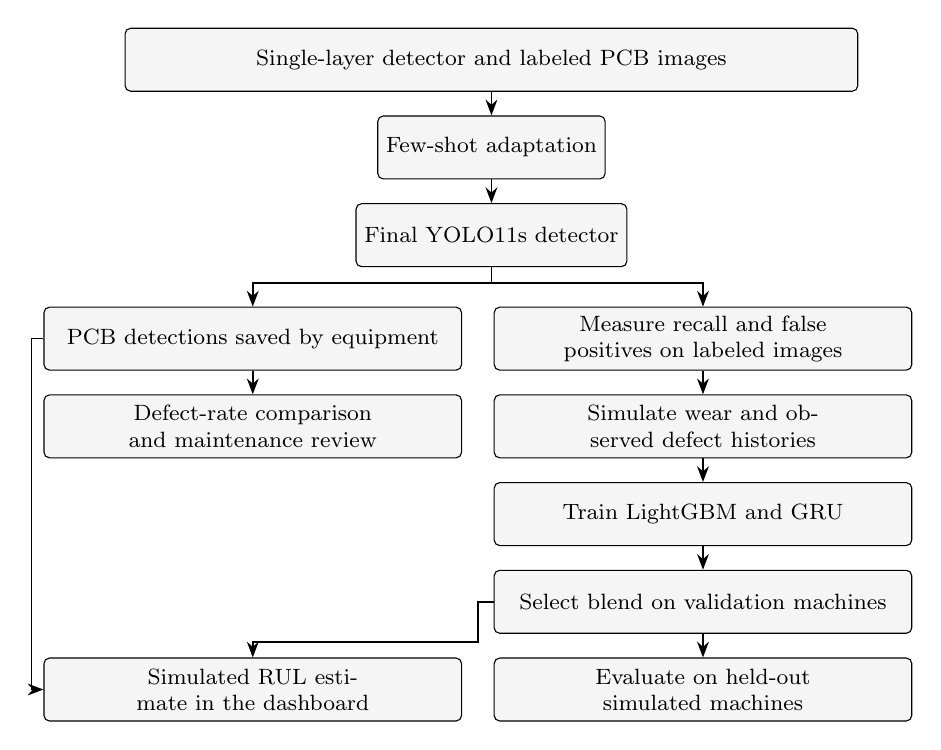
\begin{tikzpicture}[pcbflow]
\node[flowbox,text width=.75\columnwidth] (source)
  {Single-layer detector and labeled PCB images};
\node[flowbox,below=of source] (adapt) {Few-shot adaptation};
\node[flowbox,below=of adapt] (detector) {Final YOLO11s detector};
\node[branch,below=5mm of detector,xshift=-.25\columnwidth] (record)
  {PCB detections saved by equipment};
\node[branch,right=4mm of record] (measure)
  {Measure recall and false positives on labeled images};
\node[branch,below=of record] (review)
  {Defect-rate comparison and maintenance review};
\node[branch,below=of measure] (simulate)
  {Simulate wear and observed defect histories};
\node[branch,below=of simulate] (train) {Train LightGBM and GRU};
\node[branch,below=of train] (blend) {Select blend on validation machines};
\node[branch,below=of blend] (test) {Evaluate on held-out simulated machines};
\node[branch] (dashboard) at (record.center |- test.center)
  {Simulated RUL estimate in the dashboard};
\draw[arrow] (source) -- (adapt);
\draw[arrow] (adapt) -- (detector);
\draw[arrow] (detector.south) -- ++(0,-2mm) -| (record.north);
\draw[arrow] (detector.south) -- ++(0,-2mm) -| (measure.north);
\draw[arrow] (record) -- (review);
\draw[arrow] (measure) -- (simulate);
\draw[arrow] (simulate) -- (train);
\draw[arrow] (train) -- (blend);
\draw[arrow] (blend) -- (test);
\draw[arrow] (blend.west) -- ++(-2mm,0) |- ([yshift=2mm]dashboard.north) -- (dashboard.north);
\draw[arrow] (record.west) -- ++(-1.5mm,0) |- (dashboard.west);
\end{tikzpicture}
\caption{Inspection and maintenance review workflow.}
\label{fig:main-workflow}
\end{figure}

\begin{figure}[!tp]
\centering
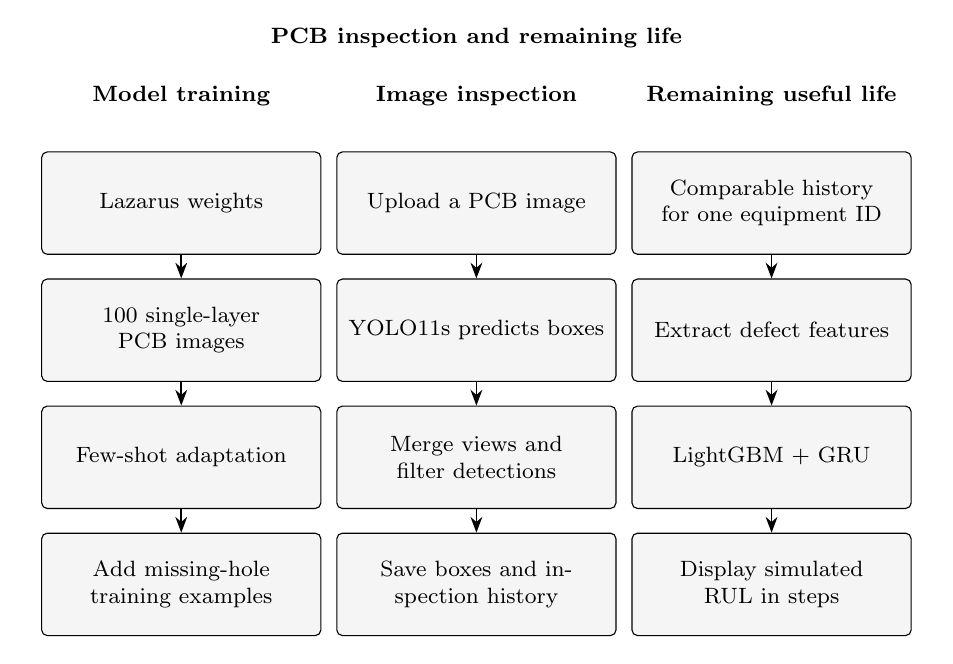
\begin{tikzpicture}[pcbflow]
\node[narrow flowheading] (training) {Model training};
\node[narrow flowheading,right=4mm of training] (inspection) {Image inspection};
\node[narrow flowheading,right=4mm of inspection] (rul) {Remaining useful life};
\node[flowtitle,above=2mm of inspection] {PCB inspection and remaining life};

\node[narrow flowbox,below=of training] (weights) {Lazarus weights};
\node[narrow flowbox,below=of weights] (source) {100 single-layer PCB images};
\node[narrow flowbox,below=of source] (adapt) {Few-shot adaptation};
\node[narrow flowbox,below=of adapt] (holes) {Add missing-hole training examples};

\node[narrow flowbox,below=of inspection] (upload) {Upload a PCB image};
\node[narrow flowbox,below=of upload] (predict) {YOLO11s predicts boxes};
\node[narrow flowbox,below=of predict] (merge) {Merge views and filter detections};
\node[narrow flowbox,below=of merge] (save) {Save boxes and inspection history};

\node[narrow flowbox,below=of rul] (history) {Comparable history for one equipment ID};
\node[narrow flowbox,below=of history] (features) {Extract defect features};
\node[narrow flowbox,below=of features] (models) {LightGBM + GRU};
\node[narrow flowbox,below=of models] (display) {Display simulated RUL in steps};

\draw[arrow] (weights) edge (source) (source) edge (adapt) (adapt) edge (holes);
\draw[arrow] (upload) edge (predict) (predict) edge (merge) (merge) edge (save);
\draw[arrow] (history) edge (features) (features) edge (models) (models) edge (display);
\end{tikzpicture}
\par\smallskip
{\footnotesize The RUL models are trained on simulated histories calibrated with detector error rates.\par}
\caption{System workflow. The detector training and image inspection paths feed a dashboard that reports defect locations and estimates simulated remaining life from inspection history.}
\label{fig:asset-01}
\end{figure}

\subsection{Dataset}

We use three PCB image datasets and a separate set of simulated equipment histories. PCB-Defect V1 supplies single-layer board images for the source detector. DefectDet V1 supplies double-layer board images for few-shot adaptation. Selected PKU-Market-PCB images supply missing-hole annotations and a separate set for measuring detector errors. We use those error measurements to simulate the defects an inspection system would record as equipment wears, providing histories for the remaining useful life (RUL) experiments.

PCB-Defect V1 contains 230 images of manufactured single-layer boards with defects produced during chemical etching. Each labeled defect has a class and a bounding box. We use 100 images to train the source detector and reuse those same images when adapting the detector to double-layer boards. The other 130 images form the single-layer development set. This set contains 821 evaluated boxes across short circuit, open circuit, spur, spurious copper, and mouse bite. The source training images contain 607 boxes across the same five classes. Reusing the original training images keeps single-layer examples in the data during adaptation. [1]

DefectDet V1 contains 268 full-board images of manufactured double-layer PCBs. The dataset authors introduced defects in the board designs before manufacturing. We use 100 labeled images from five filename groups for few-shot adaptation and reserve 148 images from nine different groups for double-layer evaluation. We use the first field of each original filename as a proxy for board design. This keeps images with the same design identifier together and leaves entire groups out of adaptation for evaluation. The preparation code checks that the two sets share no exact image files. The remaining 20 images are unused. The 100 adaptation images contain 392 boxes, and the 148 evaluation images contain 591 boxes. Both sets cover short circuit, open circuit, spur, and spurious copper. [2]

Both Mendeley datasets provide bounding boxes in COCO format. For training, we use YOLO annotations, which express the box center, width, and height relative to the image dimensions. We align class names across datasets so that a label such as open circuit has the same meaning in the source and target data. The evaluation covers the classes annotated in each prepared set. We evaluate mouse bite on the single-layer development set. Missing pad is a category in the published datasets, while missing hole is trained and evaluated using the separate PKU annotations.

For missing-hole training, we add 180 PKU images containing 375 labeled missing-hole boxes. The training images come from seven PCB layouts. Layouts 06 and 10 provide the primary missing-hole evaluation set, with 93 images and 76 labeled missing holes. We keep both layouts out of the missing-hole training set. The same 93 images include annotations for the other five defect classes, so we use them to measure detector errors for all six classes when preparing the RUL data. That calibration uses a confidence threshold of 0.25 and matches predictions to reference boxes of the same class at a minimum intersection over union of 0.50.

Each simulated equipment history starts with zero accumulated damage. At every inspection step, a positive random increment adds to that damage. The simulator records failure at the first step when cumulative damage reaches one. The target remaining life at any earlier step is the number of steps until that threshold is reached. We cap the training target at 150 inspection steps to focus the prediction on the period closer to simulated failure.

The simulated detector can miss a defect or add a false detection. For each class, the simulator uses the measured recall to determine which generated defects are detected. It also samples additional false detections using the measured average number of false positives per image for that class. Each simulated inspection records counts for the six defect classes, total and maximum detected box area, mean detection confidence, and a weighted defect count. The simulator generates area and confidence values. The recorded counts reflect both the underlying defect process and the errors expected from the detector calibration.

We generate 900 simulated machine histories and assign 600 to training, 150 to validation, and 150 to testing. All inspections from a machine stay in the same split. We use the training machines to fit the models, the validation machines to select the ensemble weights, and the test machines to measure final performance. The recorded inspection histories are the inputs to the RUL models. We score the predictions against remaining life calculated from the simulated failure times.

\subsection{Defect Detection Architecture}

We used Ultralytics YOLO11s to locate six types of PCB defects in inspection images: short circuit, open circuit, mouse bite, spur, spurious copper, and missing hole. The application uses one trained detector for all six classes. Each detection includes the defect class, a bounding box, and a confidence score. Fig.~\ref{fig:asset-02} shows the YOLO11 architecture [4] and the application’s inference steps.

\subsubsection{Backbone}

The backbone extracts features from the PCB image at several levels of detail. Convolutional layers reduce the spatial dimensions of the feature maps, and C3k2 blocks process them. The deepest stage uses spatial pyramid pooling and an attention block to incorporate information from a wider area of the image. The backbone passes features at several scales to the neck.

\subsubsection{Feature Fusion Neck}

The neck combines fine spatial detail from earlier layers with broader context from deeper layers. It upsamples deeper feature maps and joins them with earlier ones, then downsamples the combined maps and joins them again at coarser scales. This produces three feature maps for detection, with strides of 8, 16, and 32 pixels relative to the model input. The finer map preserves more detail for small defects, while the coarser maps provide context from a larger area.

\subsubsection{Detection Head}

At each of the three scales, the detection head uses one branch to predict bounding boxes and another to predict defect classes. The application returns the final box coordinates in pixels on the original image and uses them to draw the defect locations on the inspection result.

\subsubsection{Inference and Post-processing}

The application runs the detector on the original image at an inference size of 1280 pixels and on a horizontally flipped copy at 1536 pixels. It maps the flipped boxes back to the original coordinates. When boxes from the two views share a class and have an intersection over union (IoU) of at least 0.50, the application merges their coordinates using confidence as the weight. The application then applies non-maximum suppression at an IoU threshold of 0.40 to remove overlapping predictions of the same class.

The same detector also processes both views at 640 pixels. Predictions at this size can recover large missing-hole boxes when the higher-resolution predictions support them. When at least three missing-hole predictions agree across resolutions, the application also checks whether other defect boxes have a same-class match at 640 pixels. The default confidence threshold is 0.325, with a minimum of 0.40 for missing-hole detections.

\begin{figure}[!tp]
\centering
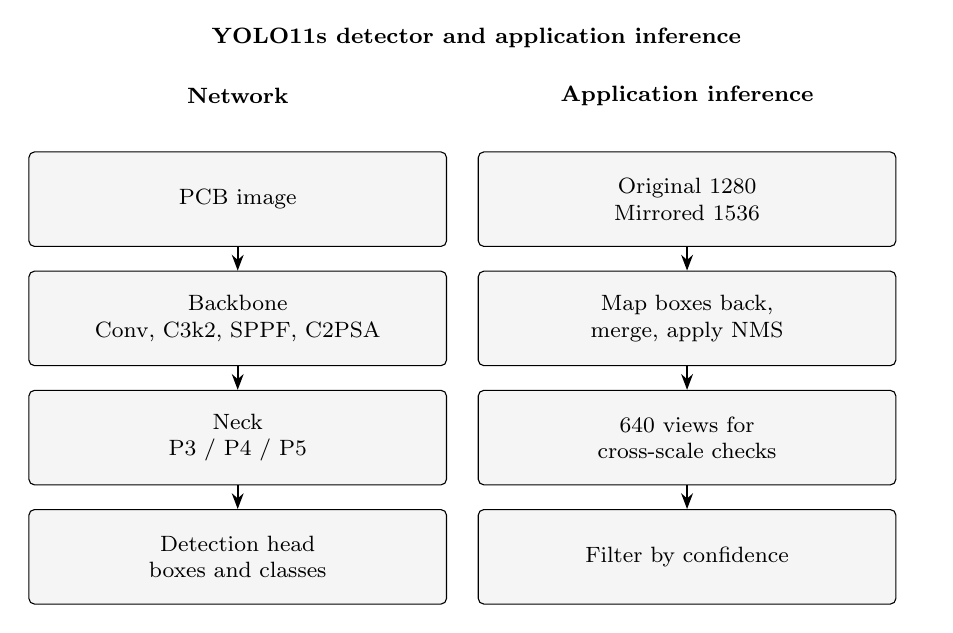
\begin{tikzpicture}[pcbflow]
\node[wide flowheading] (network) {Network};
\node[wide flowheading,right=6mm of network] (inference) {Application inference};
\node[flowtitle,above=2mm of network,xshift=.25\columnwidth]
  {YOLO11s detector and application inference};

\node[wide flowbox,below=of network] (image) {PCB image};
\node[wide flowbox,below=of image] (backbone) {Backbone\\Conv, C3k2, SPPF, C2PSA};
\node[wide flowbox,below=of backbone] (neck) {Neck\\P3 / P4 / P5};
\node[wide flowbox,below=of neck] (head) {Detection head\\boxes and classes};

\node[wide flowbox,below=of inference] (views) {Original 1280\\Mirrored 1536};
\node[wide flowbox,below=of views] (merge) {Map boxes back,\\merge, apply NMS};
\node[wide flowbox,below=of merge] (checks) {640 views for\\cross-scale checks};
\node[wide flowbox,below=of checks] (filter) {Filter by confidence};

\draw[arrow] (image) edge (backbone) (backbone) edge (neck) (neck) edge (head);
\draw[arrow] (views) edge (merge) (merge) edge (checks) (checks) edge (filter);
\end{tikzpicture}
\par\smallskip
{\footnotesize The same checkpoint processes every view. NMS IoU = 0.40. Default cutoff = 0.325, missing hole minimum = 0.40.\par}
\caption{YOLO11s architecture and inference. The detection head operates on three feature scales. The app merges original and mirrored predictions and uses 640-pixel views for cross-resolution checks.}
\label{fig:asset-02}
\end{figure}

\noindent\textbf{Algorithm 1. Detect PCB defects}\par
Input: PCB image, final checkpoint and confidence cutoff.
\begin{enumerate}
\item Predict on the original image at size 1280 and on its horizontal flip
  at size 1536. Map the flipped boxes back to the original coordinates.
\item Pair same-class boxes with IoU of at least 0.50, highest overlap first.
\item Average paired coordinates using confidence as the weight. Use the mean
  score for a pair and multiply unmatched scores by 0.75.
\item Apply class-aware non-maximum suppression at IoU 0.40.
\item Predict on both views at size 640. Use these boxes to recover large
  missing-hole candidates with support at the higher resolution.
\item If at least three higher-resolution hole boxes have support at 640,
  keep other defect boxes only when the lower scale supports their class
  and location. Apply confidence filters before returning the boxes.
\end{enumerate}
\noindent Output: Class, confidence and original-image bounding box for each detection.

\textbf{Excerpt 1. Confidence-weighted box fusion}

Source: src/backend/mirror\_merge.py, lines 22 to 29

\begin{Verbatim}[fontsize=\scriptsize,breaklines=true,breakanywhere=true]
    views = torch.stack((original[a], mirrored[b]))
    scores = views[:, 4]
    box = (views[:, :4] * scores[:, None]).sum(dim=0) / scores.sum()
    fused.append(torch.cat((box, scores.mean().reshape(1), views[0, 5:6])))
unmatched = torch.cat((original[~used_left], mirrored[~used_right]))
unmatched[:, 4] *= .75
candidates = torch.cat((torch.stack(fused), unmatched)) if fused else unmatched
keep = batched_nms(candidates[:, :4], candidates[:, 4], candidates[:, 5], nms_iou)[:max_det]
\end{Verbatim}

\subsection{Few-Shot Adaptation}

\subsubsection{Single-layer base model}

We first trained YOLO11s on 100 labelled single-layer PCB images from PCB-Defect. This stage produced a detector for five defects: short circuit, open circuit, mouse bite, spur, and spurious copper. Each double-layer adaptation run started from the same checkpoint.

\subsubsection{Adaptation to double-layer PCBs}

In the first run, we adapted the detector with 50 labelled double-layer images from DefectDet and 50 images from the original single-layer training set. In the second run, we kept those 50 double-layer images and added another 50 from the same training groups. A third run kept the 100 double-layer images fixed and increased the single-layer examples from 50 to 100. Reusing the single-layer images gave the detector examples from both board types during adaptation. The 50- and 100-image budgets count the total number of double-layer images used for training. Each image could contain multiple labelled defects.

All three runs used 30 epochs, an input size of 1280 pixels, and AdamW with an initial learning rate of 0.0002. All layers remained trainable. Because the larger training sets produced more batches per epoch, the number of training updates varied across runs. We compared the checkpoints on 148 double-layer images from groups excluded from training and checked performance on a separate 130-image single-layer development set. The double-layer comparison covered four annotated classes, and the single-layer comparison covered five.

\subsubsection{Adding missing-hole detection}

We extended the adapted detector to recognize missing hole as a sixth class. Starting from the checkpoint trained with 100 double-layer and 100 single-layer images, we kept those 200 images and added 180 labelled PKU images containing 375 missing-hole boxes. We trained this combined set for 20 epochs with an initial learning rate of 0.0001. We reserved PKU layouts 06 and 10 during training and used their predictions to assess missing-hole detection and select its confidence threshold. The application uses the resulting six-class checkpoint.

\noindent\textbf{Algorithm 2. Few-shot adaptation}\par
Input: Lazarus YOLO11s weights; labelled PCB-Defect, DefectDet and PKU images.
\begin{enumerate}
\item Train the source detector on 100 single-layer PCB-Defect images.
\item Use the same source checkpoint to start three independent adaptation runs.
  Run A uses 50 target images and 50 original source images.
  Run B uses 100 target images and the same 50 source images.
  Run C uses the same 100 target images and all 100 source images.
\item Train each adaptation run for 30 epochs at an image size of 1280.
\item Compare the checkpoints on the same single-layer and double-layer sets.
\item Start with Run C. Add 180 labelled PKU images to the same 200 images
  and continue training for 20 epochs to add the missing-hole class.
\end{enumerate}
\noindent Output: One detector checkpoint with six defect classes.

\subsection{Remaining Useful Life Estimation}

\subsubsection{Simulated inspection histories}

We generated inspection histories for 900 simulated units. At each step, damage increased by a random amount drawn from a gamma distribution. A unit failed when its accumulated damage first reached 1. The remaining useful life (RUL) at each step was the number of inspection steps until that point, capped at 150 for model training. We assigned entire histories to one split each: 600 units for training, 150 for validation, and 150 for testing.

To simulate missed defects and false detections, we ran the six-class PCB detector on 93 annotated PKU images at a confidence threshold of 0.25. We matched predictions to annotations of the same class at an IoU of at least 0.50 and measured recall and false positives per image for each class. The simulator used these rates to sample which defects were detected and how many false detections to add. Each inspection step recorded six defect counts, total and maximum bounding-box area, mean detection confidence, and a severity-weighted defect count.

For each simulated unit, the damage starts at \(D_0=0\) and increases at every inspection step:
\begin{equation}
\begin{aligned}
L &\sim \operatorname{Uniform}(400,1200),\\
D_t &= D_{t-1}+\Delta D_t,\\
\Delta D_t &\sim \operatorname{Gamma}\!\left(0.8,\frac{1}{0.8L}\right).
\end{aligned}
\end{equation}

Here, \(L\) sets the unit's expected lifetime, and the second Gamma parameter is the scale. The simulated failure step \(T\), the true remaining life \(R_t\), and the normalized training target \(y_t\) are:
\begin{equation}
\begin{aligned}
T &= \min\{t:D_t\geq 1\},\\
R_t &= T-t,\qquad
y_t = \frac{\min(R_t,150)}{150}.
\end{aligned}
\end{equation}

For defect class \(c\), the simulator generates the true count \(N_{c,t}\) and then applies the measured detector recall \(r_c\) and false positives per image \(f_c\):
\begin{equation}
\begin{aligned}
N_{c,t}&\sim\operatorname{Poisson}\!\left(m[b_c+a_cD_t^2]\right),\\
X_{c,t}&=B_{c,t}+F_{c,t},\\
B_{c,t}&\sim\operatorname{Binomial}(N_{c,t},r_c),\\
F_{c,t}&\sim\operatorname{Poisson}(f_c).
\end{aligned}
\end{equation}

Here, \(m\) is the unit-specific rate multiplier, \(b_c\) is the base defect rate, \(a_c\) controls how the rate grows with damage, and \(X_{c,t}\) is the observed count.

\subsubsection{Model training}

We trained two models on the inspection histories. LightGBM used rolling means, standard deviations, and trends over the latest 10, 30, and 100 steps, along with cumulative counts, moving averages, and elapsed time. The gated recurrent unit (GRU) used up to 100 recent inspection observations. The GRU learned to predict both RUL and simulated damage during training. Its inputs were the inspection observations and elapsed time. Both models used scaling statistics fitted on the training units. Each prediction used only information available through the current step.

The GRU predicts the normalized RUL and the simulated damage. Its loss combines the two prediction errors:
\begin{equation}
\begin{aligned}
\mathcal L_{\mathrm{GRU}}
={}&\operatorname{Huber}(\hat y_t,y_t)\\
&+0.5\,\operatorname{Huber}\!\left(\hat D_t,\min(D_t,1)\right).
\end{aligned}
\end{equation}

The damage value is used as an auxiliary training target. The model inputs are the inspection observations and elapsed time.

\subsubsection{Final prediction and application}

We averaged the predictions from five trained models of each type. Validation error determined the final combination of 20\% LightGBM and 80\% GRU. For estimates below 135 steps, we smoothed the predicted failure time using the current and earlier predictions, then converted it back to remaining steps. We limited final estimates to 0–150 inspection steps. We evaluated the completed model on the reserved test units after fixing the model settings.

The final model combines the mean predictions from the five LightGBM models and the five GRUs. The factor of 150 converts the normalized prediction back to inspection steps:
\begin{equation}
\hat R_t^{\,\mathrm{raw}}
=150\left(0.20\,\overline{\hat y}_{\mathrm{LightGBM},t}
+0.80\,\overline{\hat y}_{\mathrm{GRU},t}\right).
\end{equation}

The smoothing step estimates the failure time as \(t+\hat R_t^{\,\mathrm{raw}}\) and updates its moving average \(S_t\). It uses the smoothed result when the raw estimate is below 135 steps:
\[
\begin{aligned}
S_t &= 0.2\left(t+\hat R_t^{\,\mathrm{raw}}\right)+0.8S_{t-1},\\
S_0 &= \hat R_0^{\,\mathrm{raw}},
\end{aligned}
\]
\begin{equation}
\hat R_t=\operatorname{clip}_{[0,150]}
\begin{cases}
S_t-t, & \hat R_t^{\,\mathrm{raw}}<135,\\
\hat R_t^{\,\mathrm{raw}}, & \text{otherwise}.
\end{cases}
\end{equation}

The application builds a history for each piece of equipment from saved single-board images. It uses one image per inspection step and requires consistent detector settings throughout the history. It displays the latest prediction in inspection steps. The RUL labels come from simulated failures, so the reported errors measure performance on simulated inspection histories. Fig.~\ref{fig:asset-03} summarizes training and evaluation.

\begin{figure}[!tp]
\centering
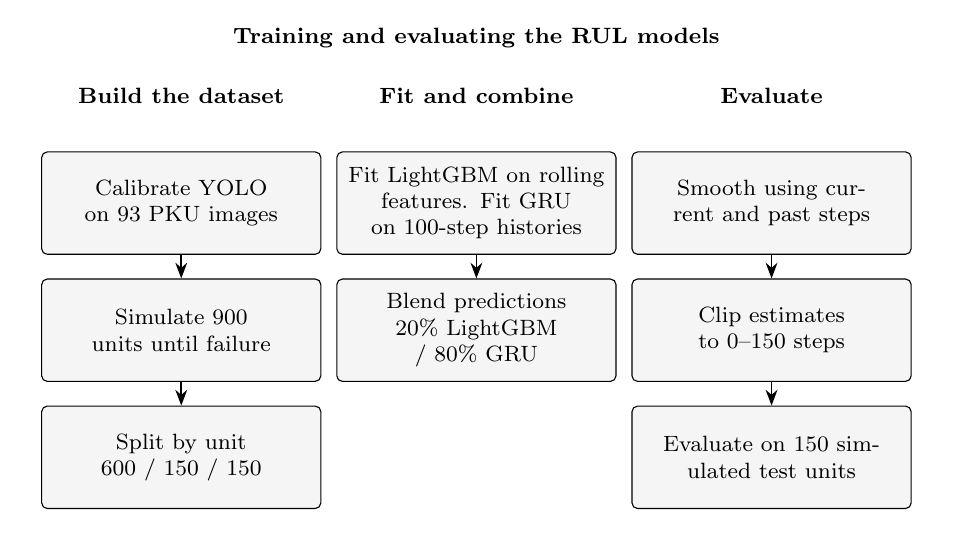
\begin{tikzpicture}[pcbflow]
\node[narrow flowheading] (dataset) {Build the dataset};
\node[narrow flowheading,right=4mm of dataset] (fit) {Fit and combine};
\node[narrow flowheading,right=4mm of fit] (evaluate) {Evaluate};
\node[flowtitle,above=2mm of fit] {Training and evaluating the RUL models};

\node[narrow flowbox,below=of dataset] (calibrate) {Calibrate YOLO on 93 PKU images};
\node[narrow flowbox,below=of calibrate] (simulate) {Simulate 900 units until failure};
\node[narrow flowbox,below=of simulate] (split) {Split by unit\\600 / 150 / 150};

\node[narrow flowbox,below=of fit] (models) {Fit LightGBM on rolling features. Fit GRU on 100-step histories};
\node[narrow flowbox,below=of models] (blend) {Blend predictions\\20\% LightGBM / 80\% GRU};

\node[narrow flowbox,below=of evaluate] (smooth) {Smooth using current and past steps};
\node[narrow flowbox,below=of smooth] (clip) {Clip estimates to 0--150 steps};
\node[narrow flowbox,below=of clip] (test) {Evaluate on 150 simulated test units};

\draw[arrow] (calibrate) edge (simulate) (simulate) edge (split);
\draw[arrow] (models) edge (blend);
\draw[arrow] (smooth) edge (clip) (clip) edge (test);
\end{tikzpicture}
\par\smallskip
{\footnotesize Five fitted members per model type. The validation split selects the blend.\par}
\caption{RUL training and evaluation. Detector errors calibrate the simulator. Unit-level splits are used to train, select and test the LightGBM-GRU ensemble. The two model families train separately and their predictions are combined.}
\label{fig:asset-03}
\end{figure}

\noindent\textbf{Algorithm 3. Simulate inspection histories}\par
Input: Per-class detector recall and false positives per image.
\begin{enumerate}
\item For each unit, sample a lifetime parameter and a defect-rate multiplier.
\item Starting at zero damage, add gamma increments until damage reaches one.
\item At each step, generate class counts from damage-dependent Poisson rates.
  Thin each count using detector recall, then add Poisson false positives.
\item Sample box areas and detection confidence scores. Record six class counts,
  total and maximum box area, mean confidence and weighted defect count.
\item Label each step with the time remaining to simulated failure. Cap and
  normalize the RUL training target. Store clipped damage as an auxiliary
  target for the GRU. Assign entire units to train, validation or test.
\end{enumerate}
\noindent Output: 600 training units, 150 validation units and 150 test units.

\noindent\textbf{Algorithm 4. Estimate remaining useful life}\par
Input: Ordered inspection observations for a unit.
\begin{enumerate}
\item Build causal rolling and cumulative features for LightGBM. Prepare the
  latest 100 observations or fewer plus elapsed time for the GRU.
\item Apply the scaling fitted on the training units.
\item Average the predictions from five LightGBM members and from five GRUs.
\item Combine the averages using weights of 0.20 and 0.80. Convert to steps.
\item Add elapsed time to estimate the failure step. Update the moving average
  with alpha 0.20. Use its value minus elapsed time when raw RUL is below 135.
\item Clip the result to the range 0 to 150.
\end{enumerate}
\noindent Output: Simulated RUL in inspection steps.

\textbf{Excerpt 2. Preparing one inspection observation}

Source: src/rul\_synthesis/ensemble\_runtime.py, lines 16 to 27

\begin{Verbatim}[fontsize=\scriptsize,breaklines=true,breakanywhere=true]
def inspection_features(detections, width, height):
    """Match the observed feature order and normalized box areas used in training."""
    counts = np.zeros(len(CLASSES), dtype=np.float32)
    areas, confidences = [], []
    for detection in detections:
        name = detection['class_name']
        counts[CLASSES.index('open' if name == 'open_circuit' else name)] += 1
        x1, y1, x2, y2 = detection['bbox']
        areas.append((min(x2, width) - min(x1, width)) * (min(y2, height) - min(y1, height)) / (width * height))
        confidences.append(detection['confidence'])
    return np.array([*counts, sum(areas), max(areas, default=0),
                     np.mean(confidences) if confidences else 0, counts @ SEVERITY], dtype=np.float32)
\end{Verbatim}

\textbf{Excerpt 3. Converting the ensemble output to inspection steps}

Source: pcb\_rul/ensemble.py, lines 15 to 27

\begin{Verbatim}[fontsize=\scriptsize,breaklines=true,breakanywhere=true]
def blend(lightgbm, gru, weight):
    return weight * lightgbm + (1 - weight) * gru


def smooth(prediction, units, step):
    raw = np.asarray(prediction, dtype=np.float64) * RUL_CAP
    result = raw.copy()
    for rows in unit_slices(units):
        failure = step[rows] + raw[rows]
        # The initial EWMA is the first estimate for this unit.
        averaged, _ = lfilter([0.2], [1.0, -0.8], failure, zi=[0.8 * failure[0]])
        result[rows] = np.where(raw[rows] < 0.9 * RUL_CAP, averaged - step[rows], raw[rows])
    return np.clip(result, 0, RUL_CAP)
\end{Verbatim}

\section{Results}

\paragraph{Evaluation Metrics}
For a predicted bounding box \(B_p\) and its ground-truth box \(B_g\), intersection over union measures how much they overlap:
\begin{equation}
\begin{aligned}
\operatorname{IoU}(B_p,B_g)&=\frac{|B_p\cap B_g|}{|B_p\cup B_g|}.\\
\operatorname{mAP}_{50}&=\frac{1}{C}\sum_{c=1}^{C}\operatorname{AP}_{c}(0.50).
\end{aligned}
\end{equation}

Here, \(C\) is the number of classes evaluated on that dataset. \(\operatorname{mAP}_{50:95}\) averages the class mean AP over ten IoU thresholds from 0.50 to 0.95 in increments of 0.05. At the chosen confidence threshold, precision is \(TP/(TP+FP)\) and recall is \(TP/(TP+FN)\).

\subsection{Defect Detection}

\subsubsection{Effect of few-shot adaptation}

Before adaptation, the single-layer model scored \textbf{81.51\% mAP50} on 130 single-layer images and \textbf{0.00\% mAP50} on 148 double-layer images. With 50 labelled double-layer images and 50 single-layer training images, the model reached \textbf{79.41\% mAP50} on the double-layer comparison set while scoring \textbf{80.34\%} on the single-layer set.

Increasing the double-layer training set to 100 images while keeping 50 single-layer images raised double-layer mAP50 to \textbf{84.93\%}, while single-layer mAP50 fell to \textbf{72.81\%}. Using all 100 original single-layer training images with the same 100 double-layer images yielded \textbf{85.20\% on single-layer images} and \textbf{83.01\% on double-layer images}. We used this checkpoint to add missing-hole detection because it performed more consistently across the two datasets. Fig.~\ref{fig:asset-07} shows the results at each training stage.

\begin{figure}[!tp]
\centering
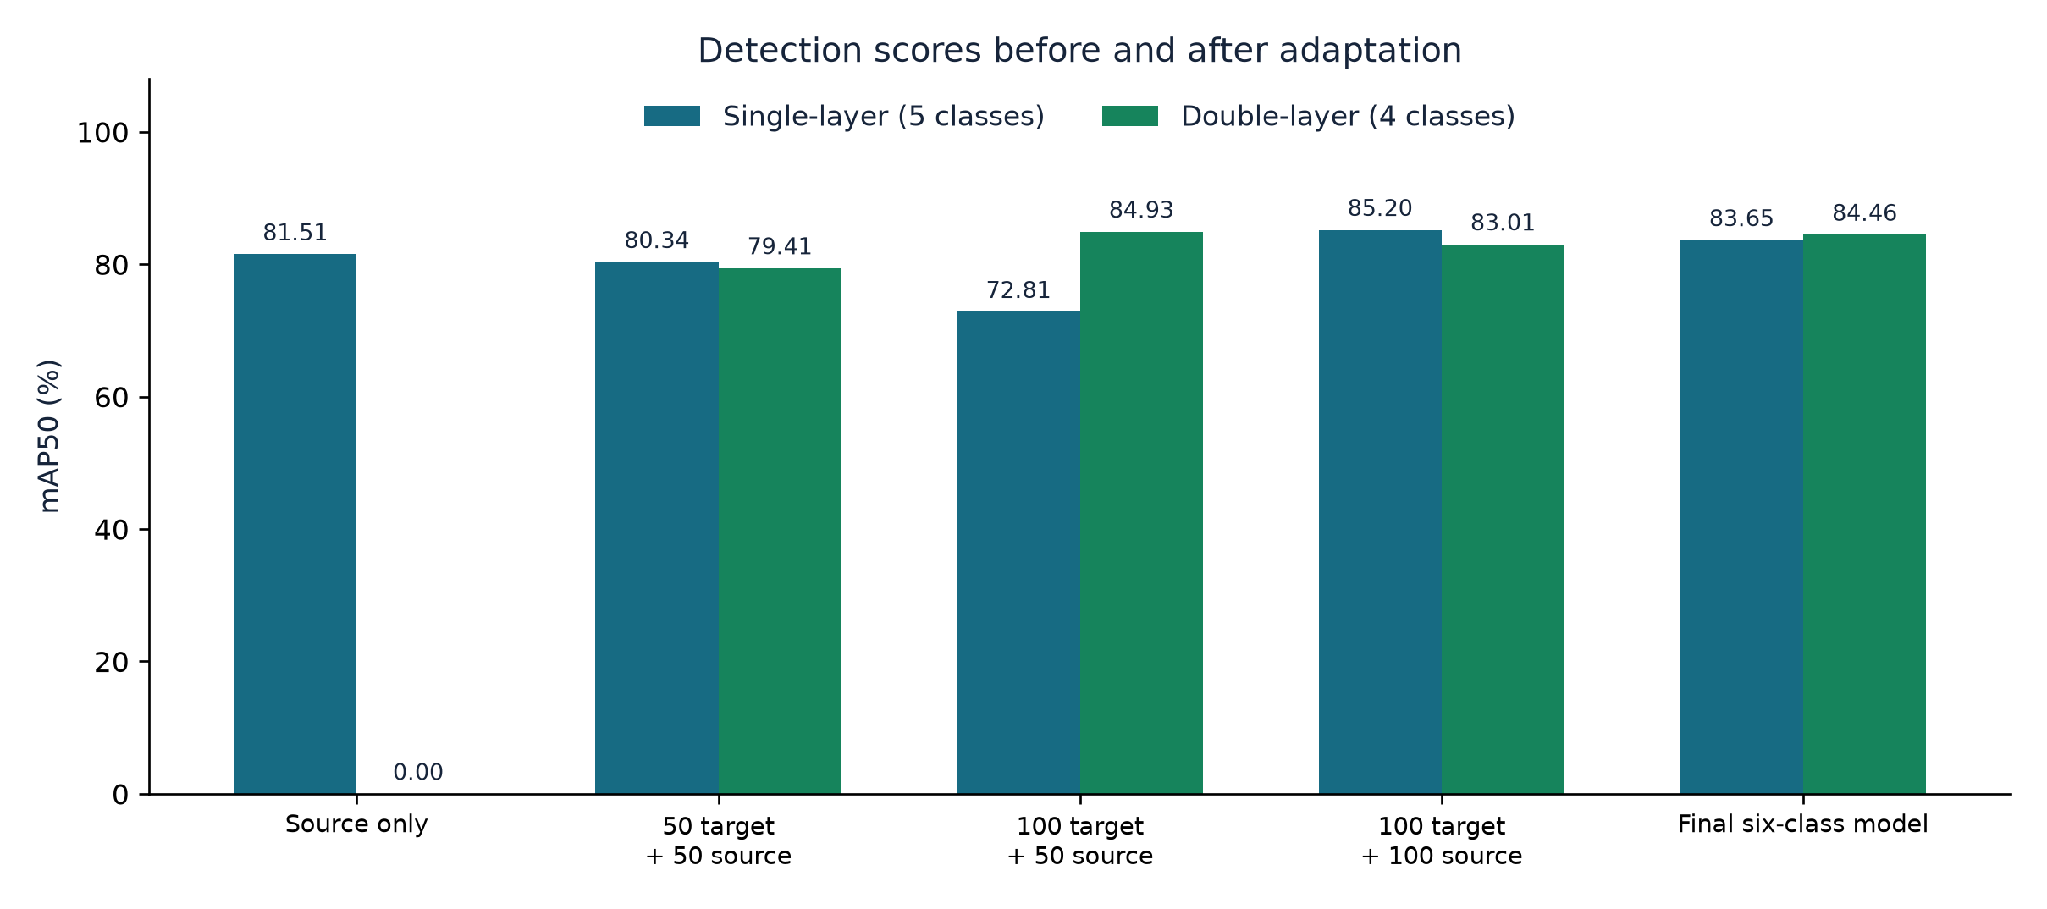
\includegraphics[width=\columnwidth,height=.43\textheight,keepaspectratio]{figures/figure-07.png}
\caption{Few-shot adaptation results. mAP50 at each training stage on the same 130 single-layer and 148 double-layer images. Counts in the labels refer to training images. The final model also includes PKU missing-hole examples.}
\label{fig:asset-07}
\end{figure}

\subsubsection{Final six-class detector}

The final checkpoint reached \textbf{83.65\% mAP50} and \textbf{38.20\% mAP50–95} across five annotated classes on the single-layer set. It reached \textbf{84.46\% mAP50} and \textbf{43.69\% mAP50–95} across four annotated classes on the double-layer set. At a confidence threshold of 0.325, precision and recall were \textbf{82.92\% and 78.08\%} on the single-layer set and \textbf{88.48\% and 78.00\%} on the double-layer set. Each set of scores covers its annotated classes. Figs.~\ref{fig:asset-04} and~\ref{fig:asset-05} show example detections. Figs.~\ref{fig:asset-08} and~\ref{fig:asset-09} show the confusion matrices, and Fig.~\ref{fig:asset-10} reports AP50 by class.

\begin{figure}[!tp]
\centering
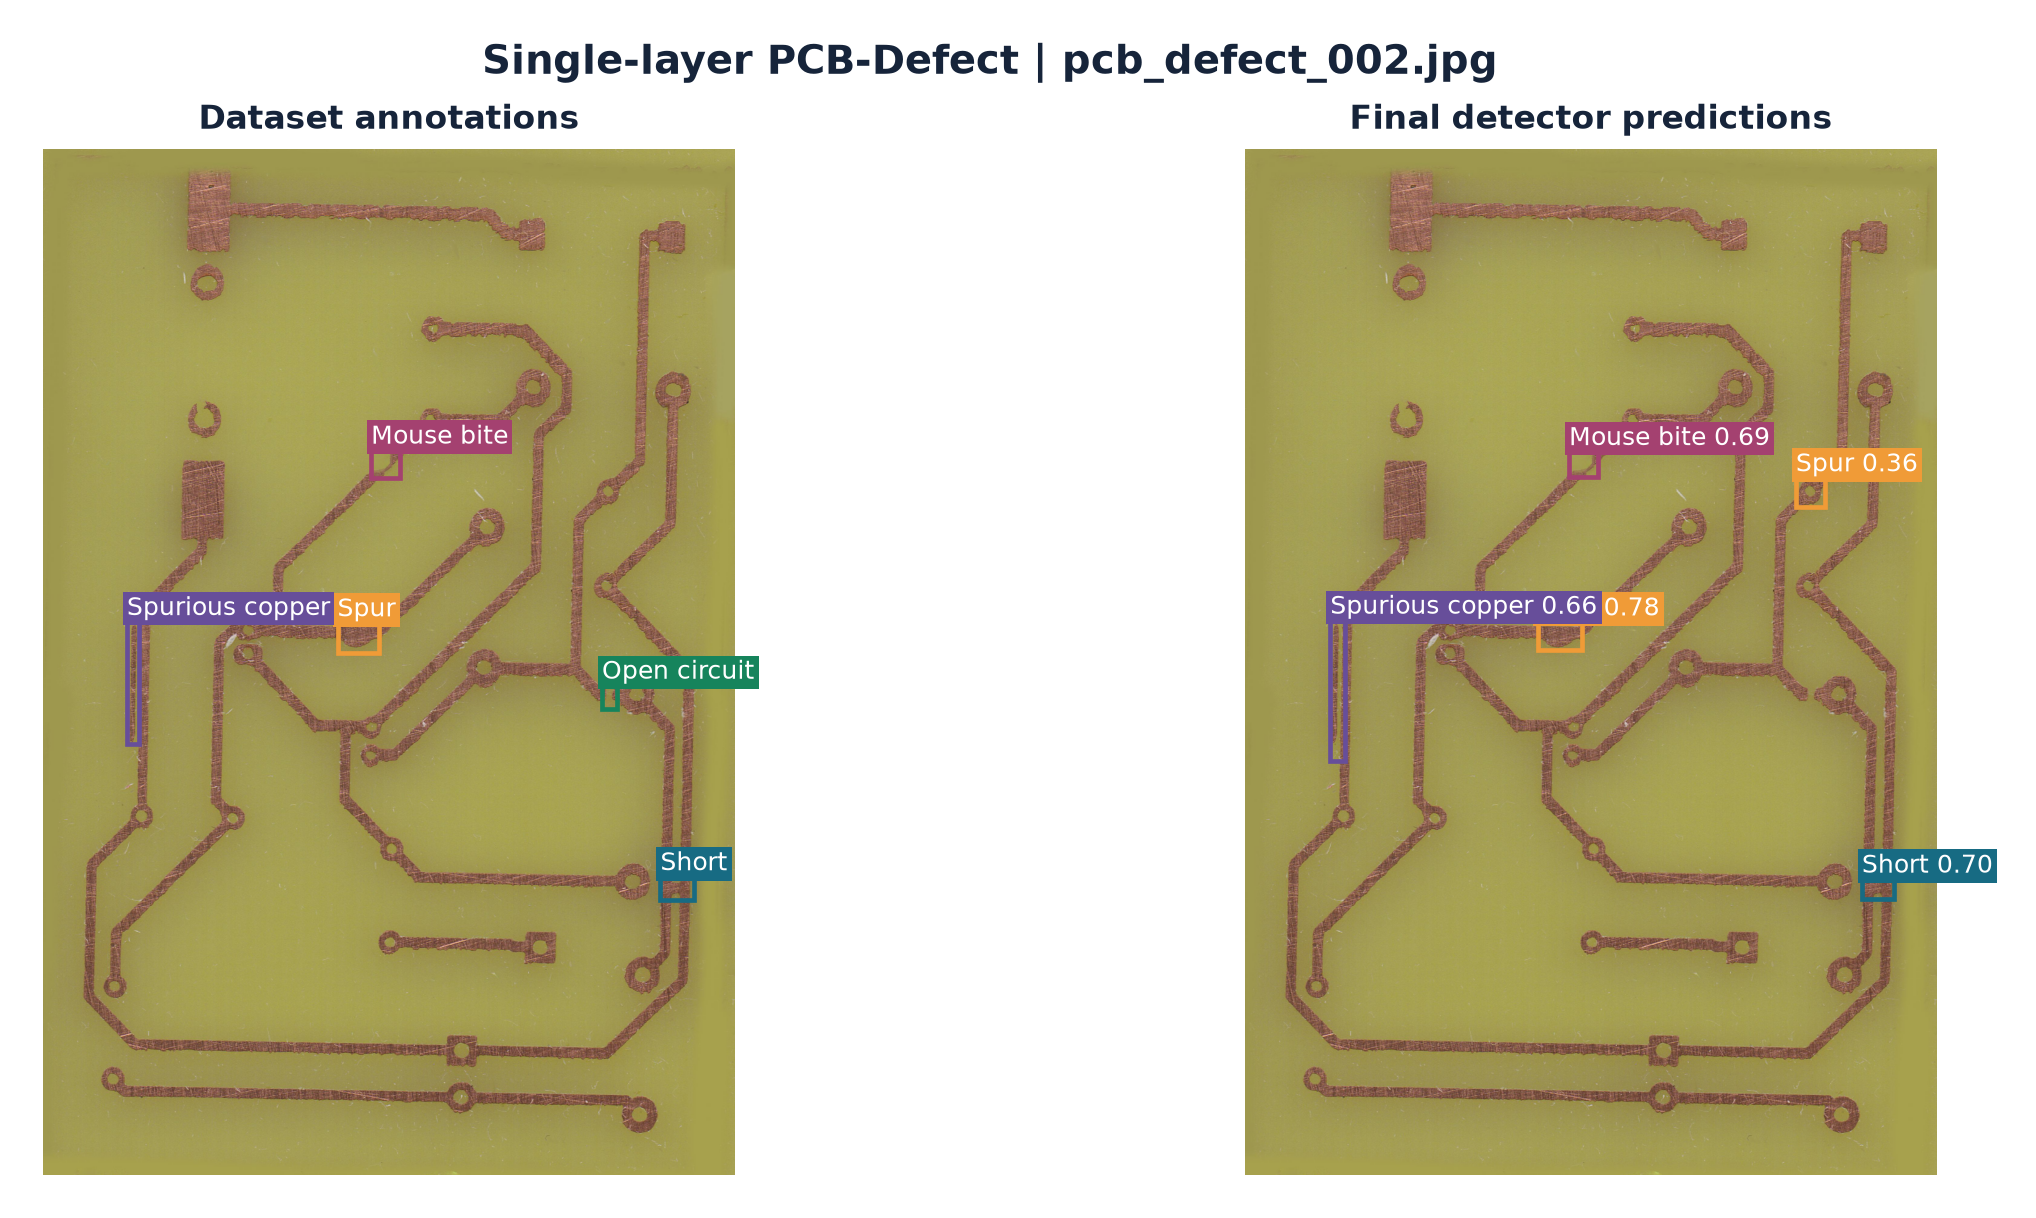
\includegraphics[width=\columnwidth,height=.43\textheight,keepaspectratio]{figures/figure-04.png}
\caption{Single-layer detection example. Dataset annotations and final detector predictions on pcb\_defect\_002.jpg, using the five scored classes. PCB-Defect V1, Rashid et al., CC BY 4.0, doi:10.17632/vdj74sngvn.1. Bounding boxes added.}
\label{fig:asset-04}
\end{figure}

\begin{figure}[!tp]
\centering
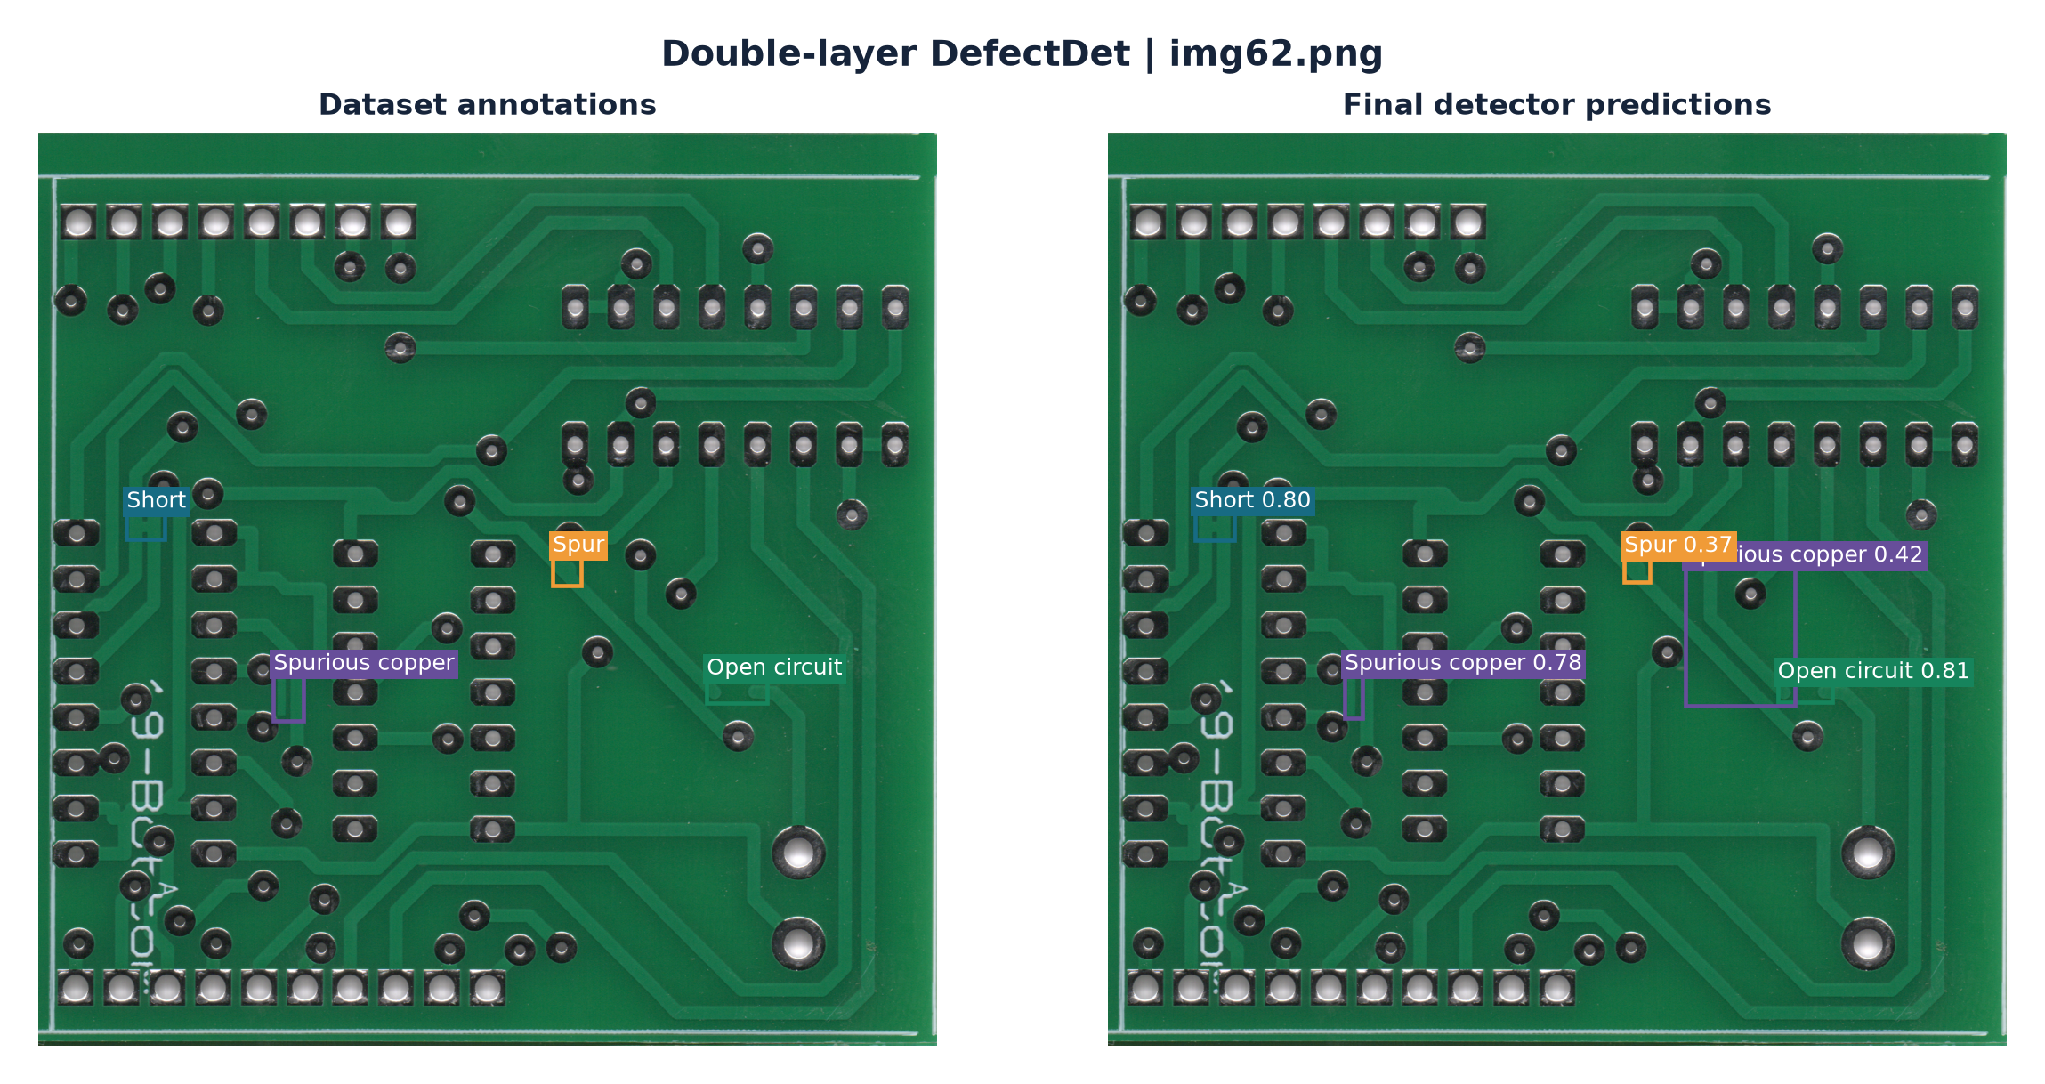
\includegraphics[width=\columnwidth,height=.43\textheight,keepaspectratio]{figures/figure-05.png}
\caption{Double-layer detection example. Dataset annotations and final detector predictions on img62.png, using the four scored classes. DefectDet V1, Azam et al., CC BY 4.0, doi:10.17632/t9d9zs3bmb.1. Bounding boxes added.}
\label{fig:asset-05}
\end{figure}

\begin{figure}[!tp]
\centering
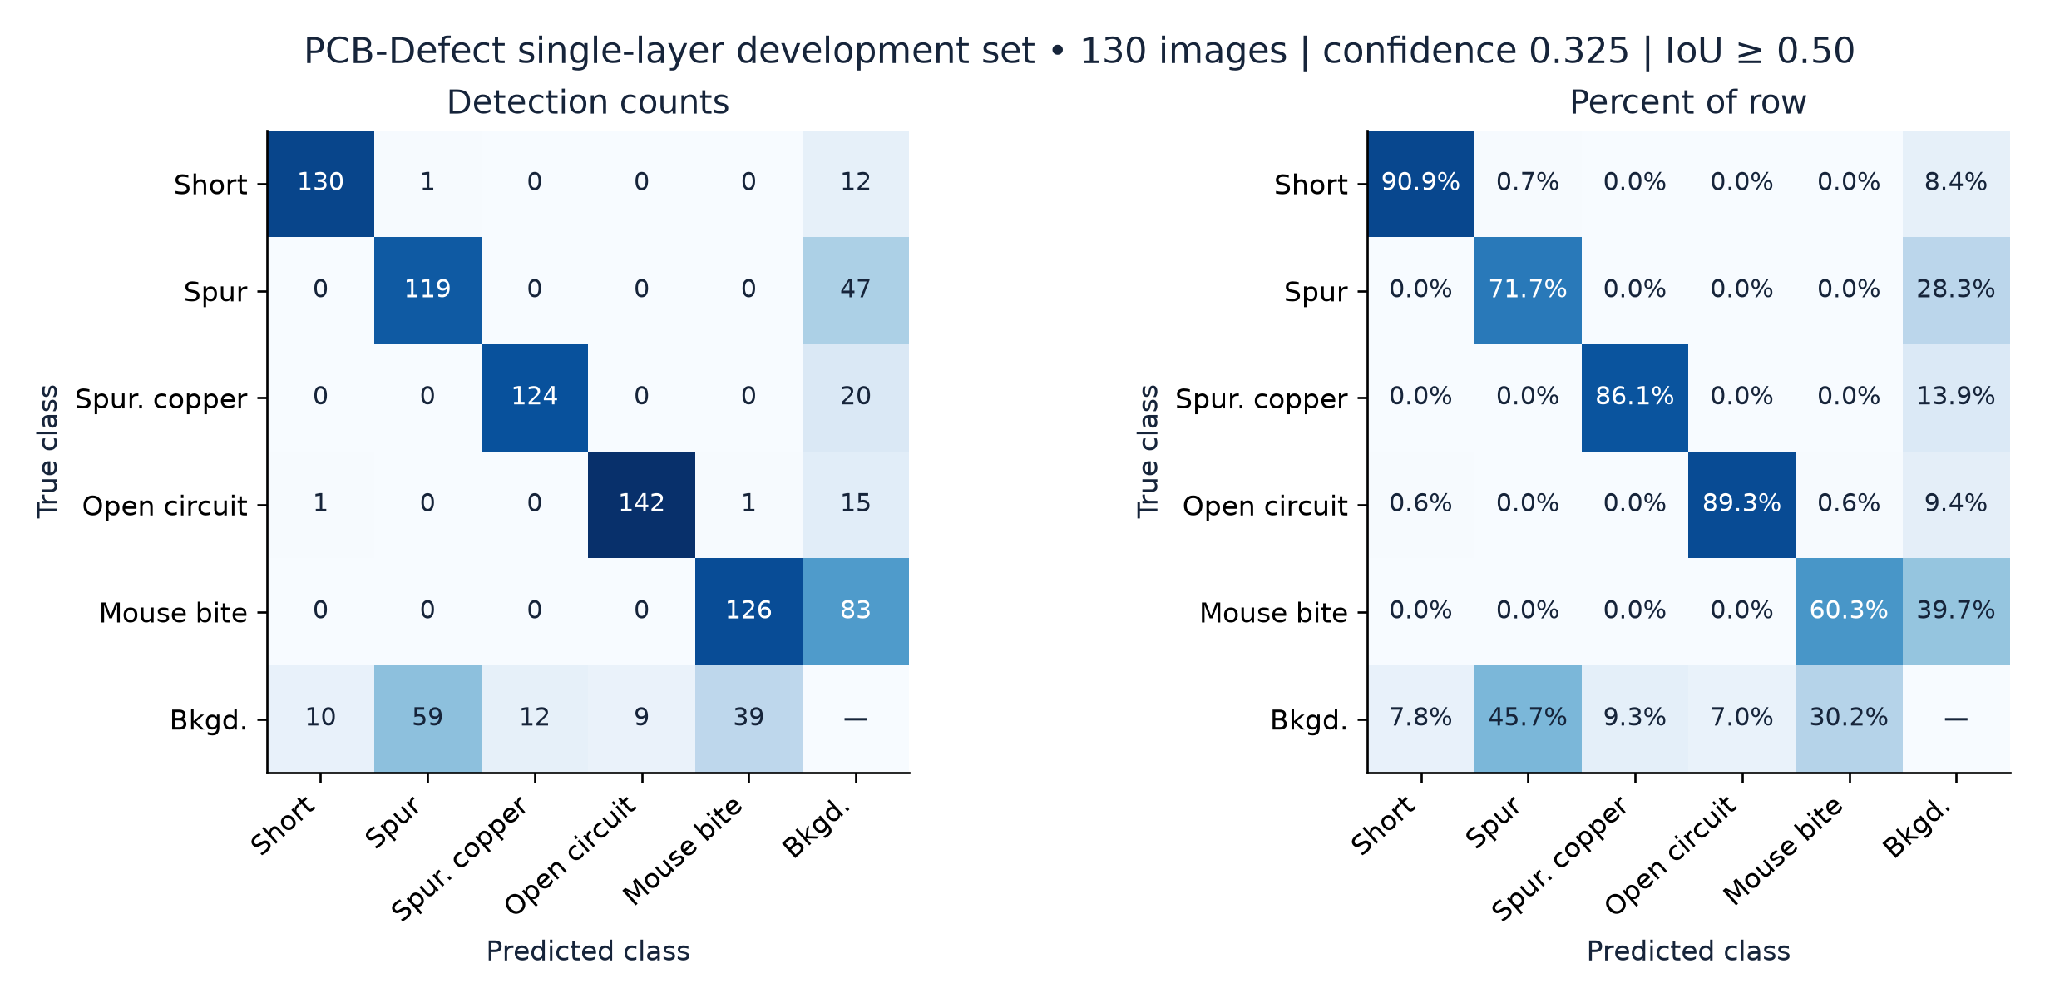
\includegraphics[width=\columnwidth,height=.43\textheight,keepaspectratio]{figures/figure-08.png}
\caption{Single-layer detection confusion matrix. Five classes on 130 PCB-Defect development images, confidence 0.325 and IoU 0.50. Rows show true classes and columns show predictions. Unmatched detections appear in the background row and missed defects in the background column.}
\label{fig:asset-08}
\end{figure}

\begin{figure}[!tp]
\centering
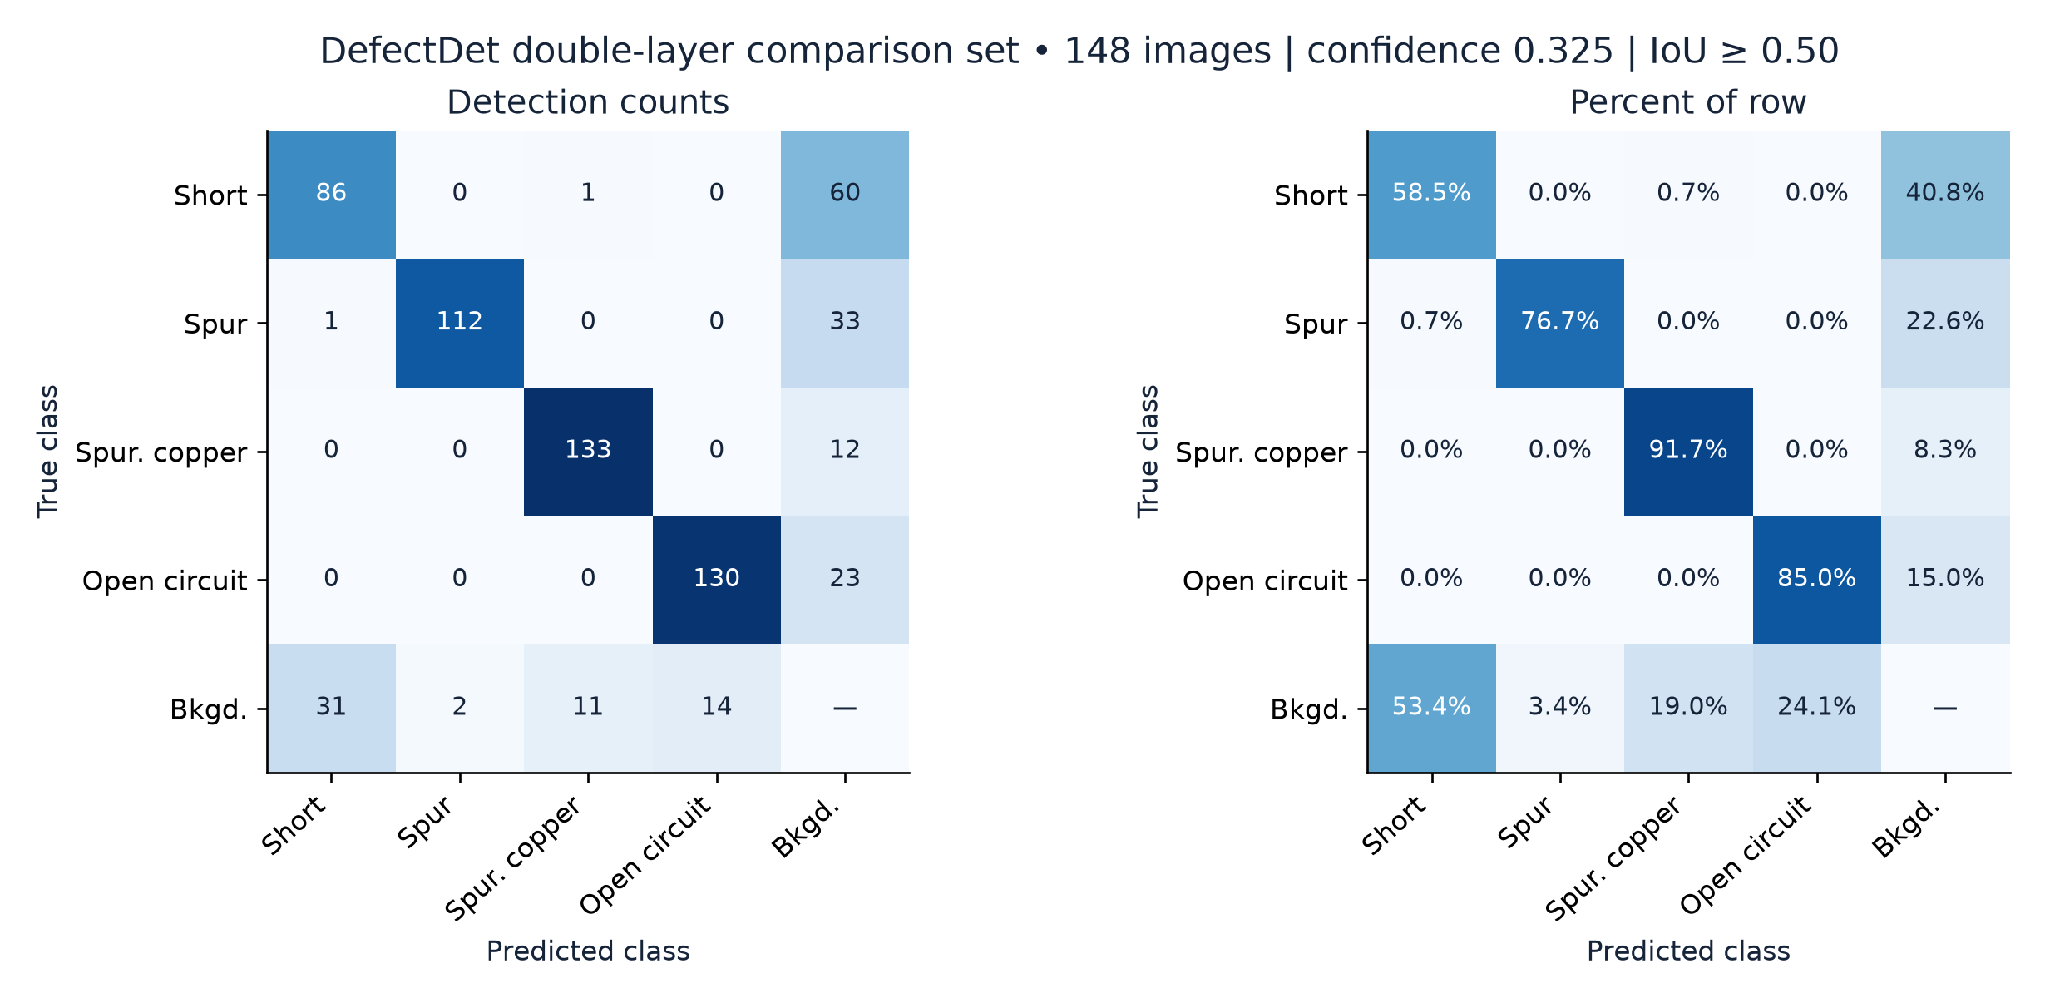
\includegraphics[width=\columnwidth,height=.43\textheight,keepaspectratio]{figures/figure-09.png}
\caption{Double-layer detection confusion matrix. Four classes on 148 DefectDet comparison images, confidence 0.325 and IoU 0.50. Rows show true classes and columns show predictions. Unmatched detections appear in the background row and missed defects in the background column.}
\label{fig:asset-09}
\end{figure}

\begin{figure}[!tp]
\centering
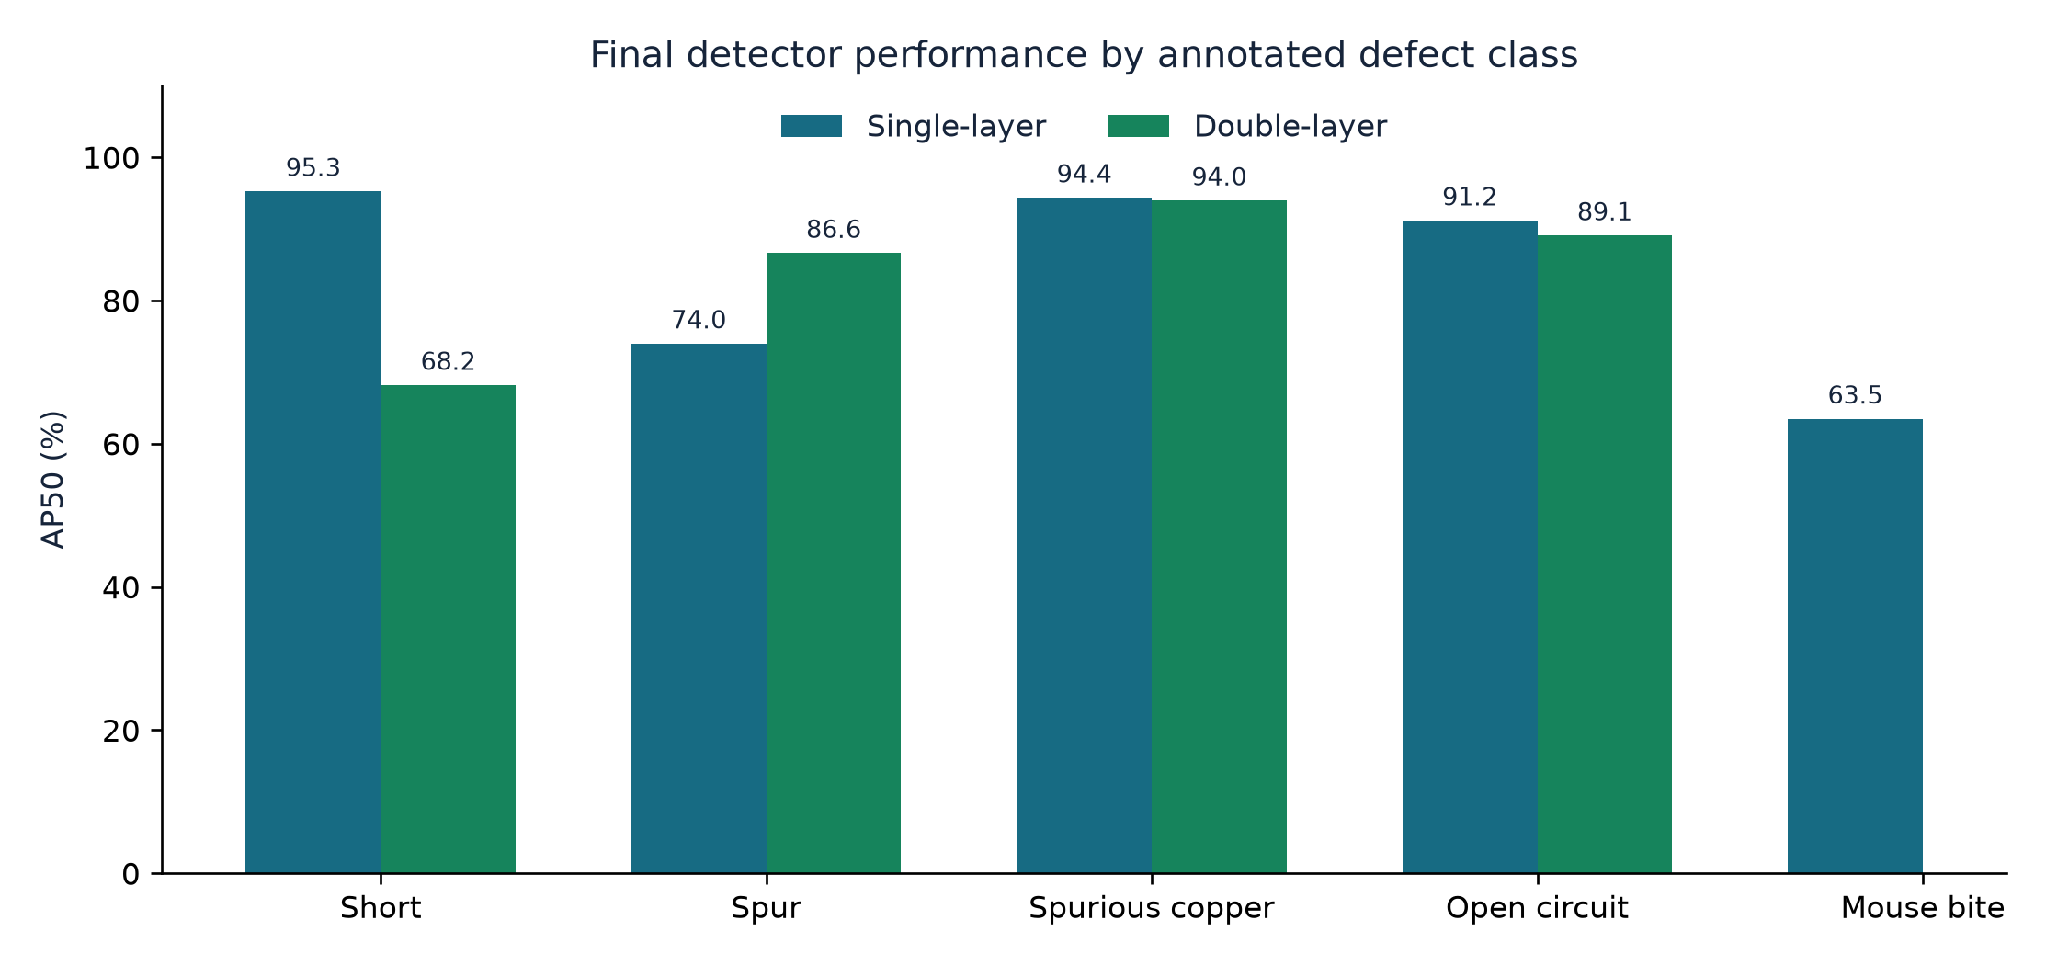
\includegraphics[width=\columnwidth,height=.43\textheight,keepaspectratio]{figures/figure-10.png}
\caption{Class-wise AP50. Final detector results by annotated defect class. Mouse bite was evaluated on the single-layer set.}
\label{fig:asset-10}
\end{figure}

\subsubsection{Missing-hole detection}

On 93 PKU images from layouts 06 and 10, missing-hole detection reached \textbf{91.87\% AP50} before the supplementary 640-pixel pass. At a confidence threshold of 0.40, the additional pass increased the number of matched detections from \textbf{69 to 72 out of 76} labelled missing holes, with zero false positives on those images. We used these layouts to choose the threshold and recovery settings. A visual review of double-layer DefectDet images found missing-hole alerts on existing holes and printed markings. DefectDet had no missing-hole annotations for calculating AP for this class. Figs.~\ref{fig:asset-06} and~\ref{fig:asset-11} show examples of matches and false alerts.

\begin{figure}[!tp]
\centering
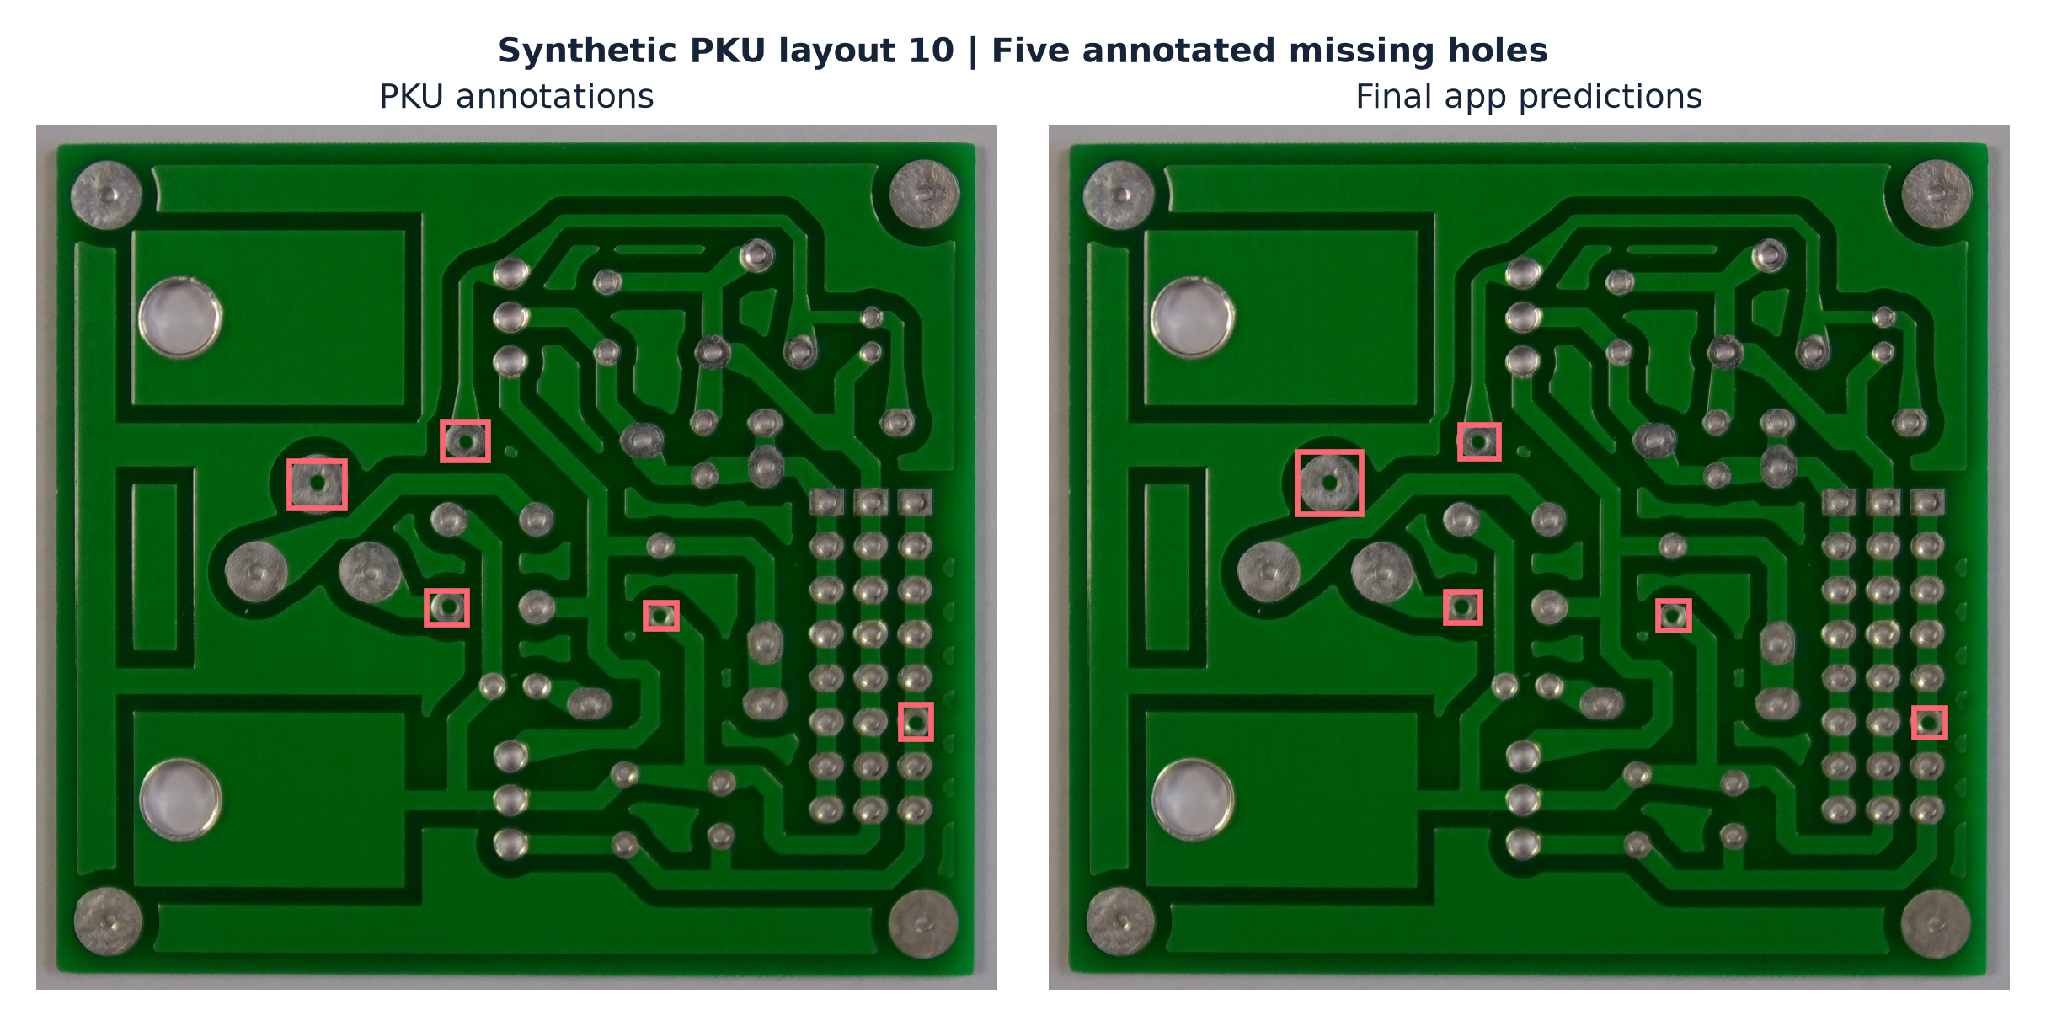
\includegraphics[width=\columnwidth,height=.43\textheight,keepaspectratio]{figures/figure-06.png}
\caption{Synthetic missing-hole example. PKU layout 10, 10\_missing\_hole\_02.jpg. The final app matched all five annotated missing holes on this example at IoU 0.50. The panels show only missing-hole boxes. Credit Huang and Wei, arXiv:1901.08204.}
\label{fig:asset-06}
\end{figure}

\begin{figure}[!tp]
\centering
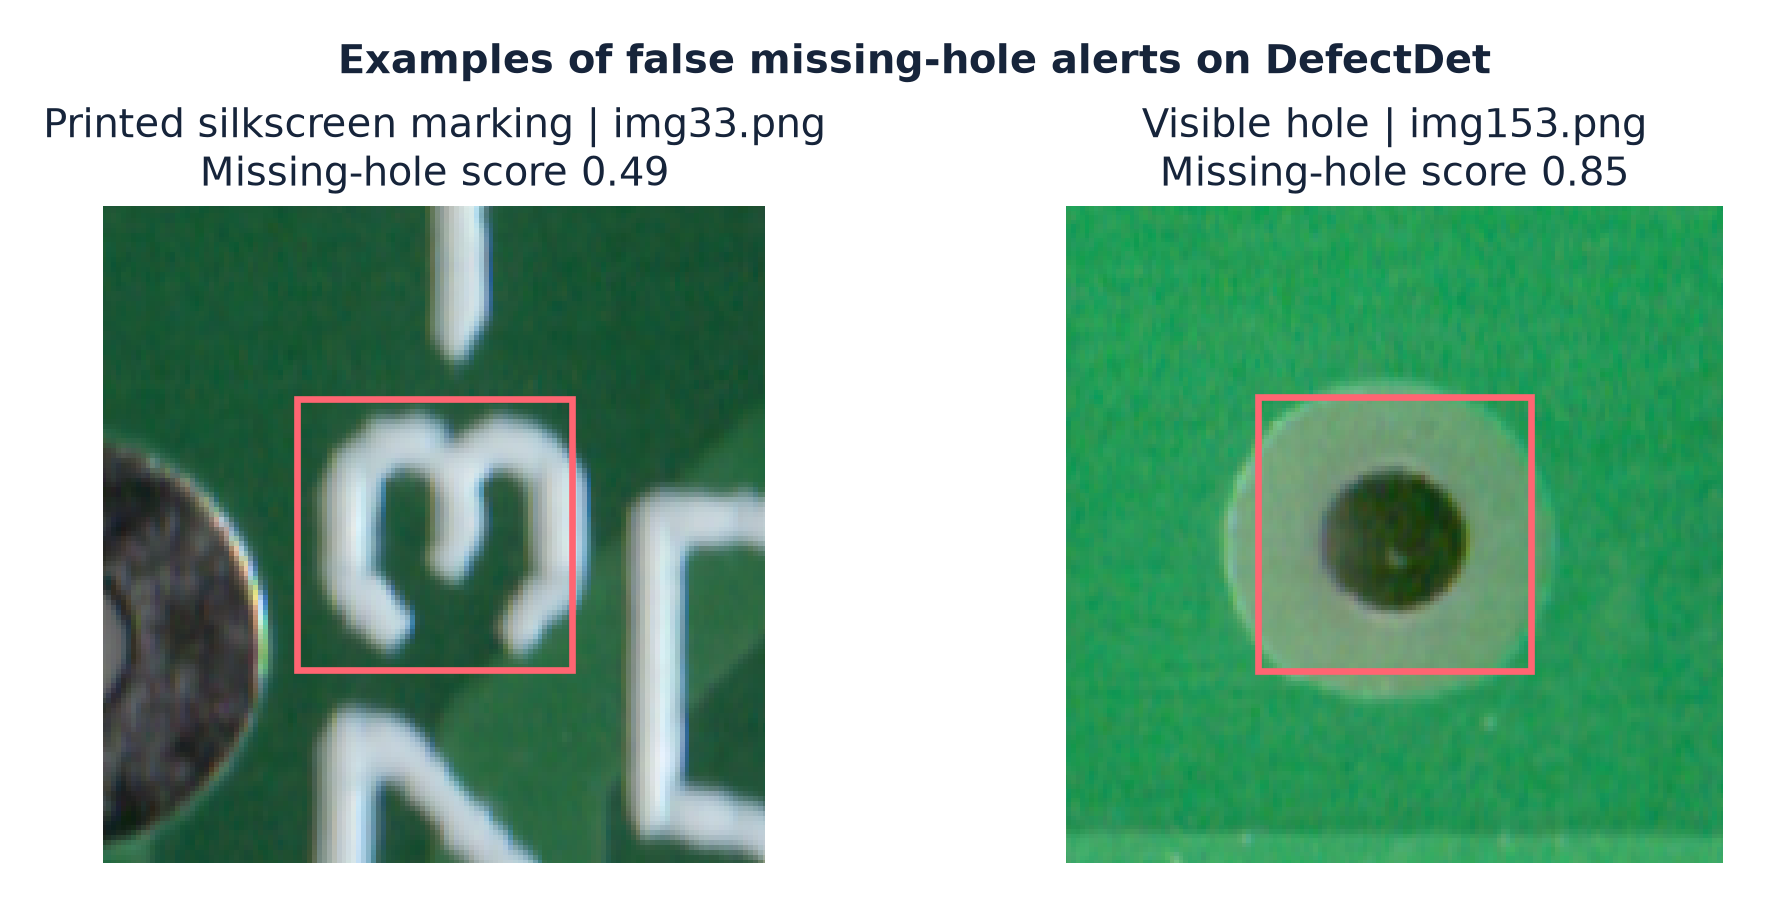
\includegraphics[width=\columnwidth,height=.43\textheight,keepaspectratio]{figures/figure-11.png}
\caption{False missing-hole alerts. Two audited DefectDet examples show detections on a printed marking and an existing hole. The audit found 29 such alerts across nine images. DefectDet V1, Azam et al., CC BY 4.0. Image crops and boxes added.}
\label{fig:asset-11}
\end{figure}

\subsection{Remaining Useful Life Results}

For \(n\) evaluated inspection steps, let \(e_i=\hat R_i-R_i^\ast\), where \(R_i^\ast\) is the capped or uncapped target used in that comparison:
\begin{equation}
\begin{aligned}
\operatorname{MAE}&=\frac{1}{n}\sum_{i=1}^{n}|e_i|,\\
\operatorname{RMSE}&=\sqrt{\frac{1}{n}\sum_{i=1}^{n}e_i^2},\\
\text{MAE as \% of cap}&=100\frac{\operatorname{MAE}}{150}.
\end{aligned}
\end{equation}

The asymmetric RUL score penalizes overestimation more heavily than underestimation of the same size. The evaluation reports both the sum and the mean of the per-step penalties:
\begin{equation}
\begin{aligned}
s_i &=
\begin{cases}
\exp(-e_i/13)-1, & e_i<0,\\
\exp(e_i/10)-1, & e_i\geq0,
\end{cases}\\
S_{\mathrm{sum}}&=\sum_{i=1}^{n}s_i,\qquad
S_{\mathrm{mean}}=\frac{S_{\mathrm{sum}}}{n}.
\end{aligned}
\end{equation}

We evaluated the RUL model on \textbf{150 simulated units}, covering \textbf{115,341 inspection steps}. Mean absolute error (MAE) measures how far predictions were from simulated remaining life on average. Root mean squared error (RMSE) gives larger errors more weight. We report both in inspection steps.

\subsubsection{Overall prediction error}

Against the \textbf{150-step capped target}, the final ensemble achieved an MAE of \textbf{3.28 steps} and an RMSE of \textbf{8.19 steps}. The MAE was \textbf{2.19\% of the 150-step cap}. The train-mean, time-only LightGBM, and ridge regression baselines had MAEs of \textbf{23.60}, \textbf{13.53}, and \textbf{9.38 steps}, respectively. LightGBM using inspection features reached \textbf{3.80 steps}, while the GRU reached \textbf{3.30 steps}. The GRU’s average error was close to the ensemble’s. Fig.~\ref{fig:asset-12} compares the models.

\subsubsection{Prediction error near failure}

Across the \textbf{7,650 inspection steps} with 50 or fewer steps remaining, the ensemble achieved an MAE of \textbf{10.58 steps} and an RMSE of \textbf{13.92 steps}. The GRU had an MAE of \textbf{10.59 steps} on those same steps. Across five seed-specific blends, the mean MAE was \textbf{3.39 \ensuremath{\pm} 0.16 steps} over all observations against the capped target and \textbf{10.86 \ensuremath{\pm} 0.38 steps} near failure.

\subsubsection{Effect of the prediction cap}

The model reports up to \textbf{150 remaining steps}. When we compared predictions with uncapped simulated remaining life across all inspection steps, the ensemble’s MAE was \textbf{283.70 steps}. This comparison includes early inspections where the simulated remaining life exceeded the model’s output range. Figs.~\ref{fig:asset-14} and~\ref{fig:asset-15} show how the cap affects error by life stage and the comparison with true RUL.


\begin{figure}[!tp]
\centering
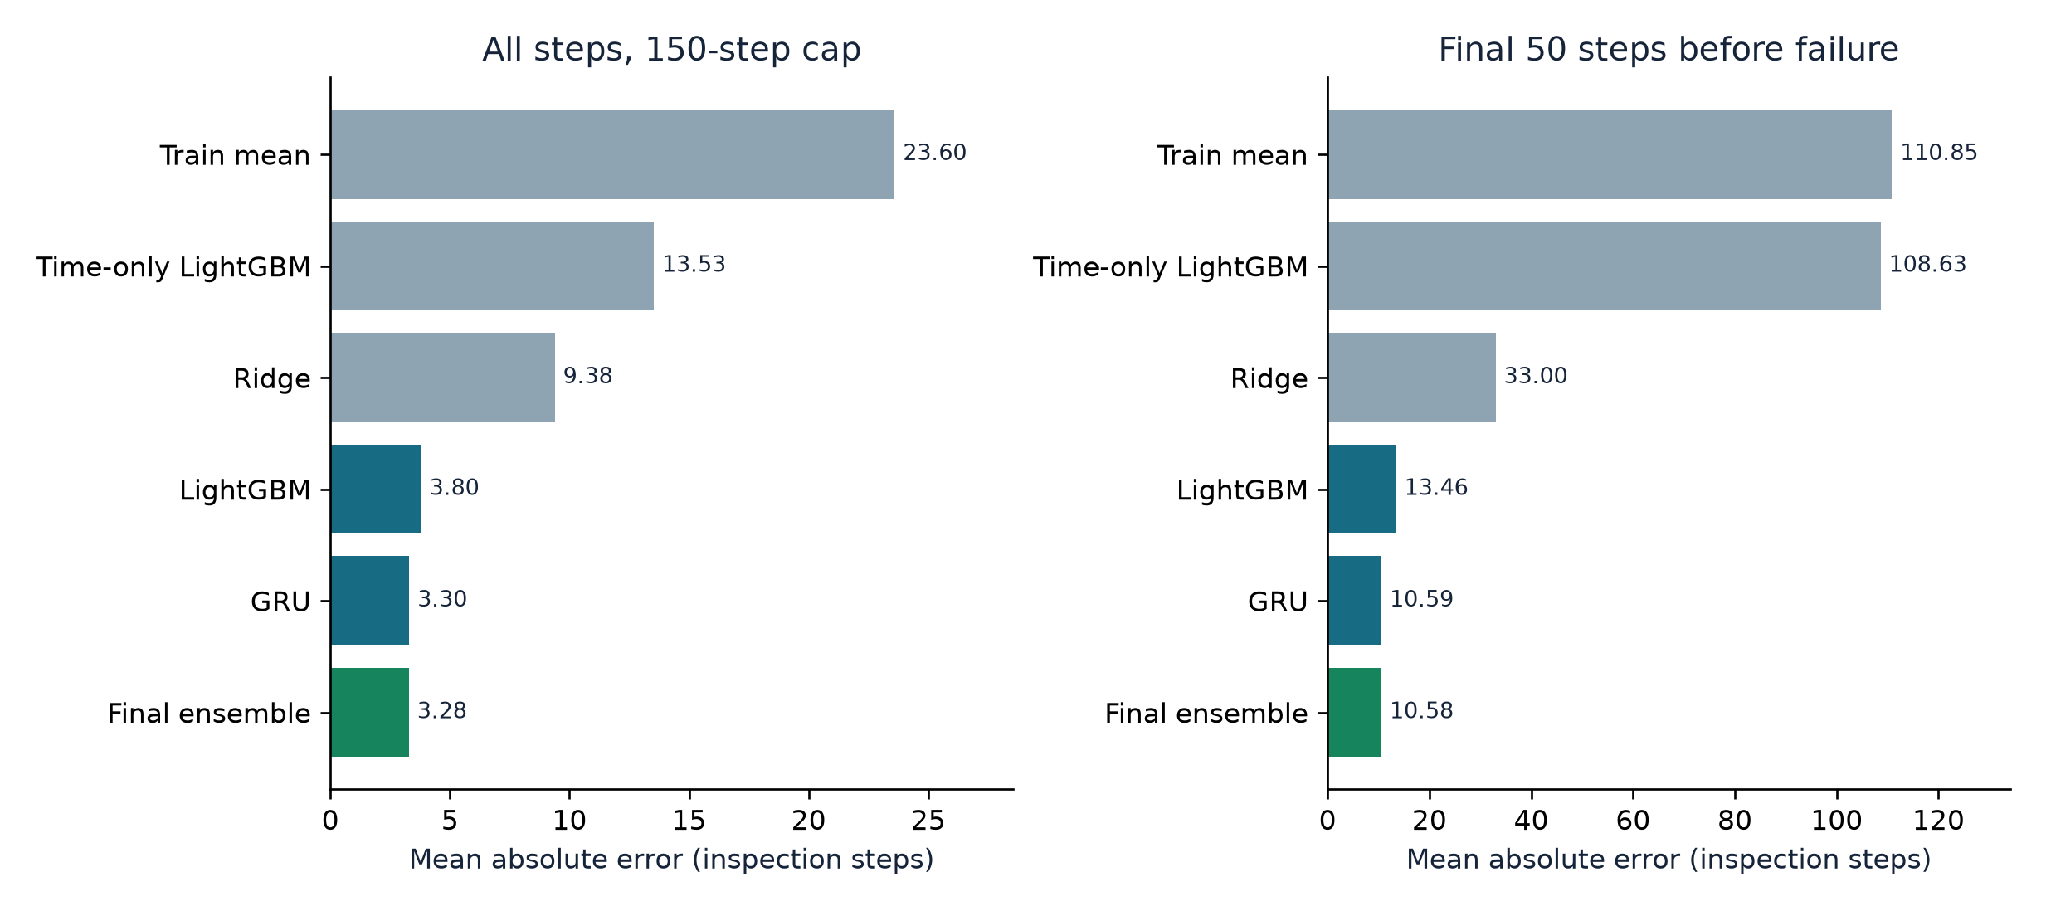
\includegraphics[width=\columnwidth,height=.43\textheight,keepaspectratio]{figures/figure-12.png}
\caption{RUL model comparison. Test mean absolute error against the 150-step capped target and during the final 50 steps before simulated failure.}
\label{fig:asset-12}
\end{figure}

\begin{figure}[!tp]
\centering
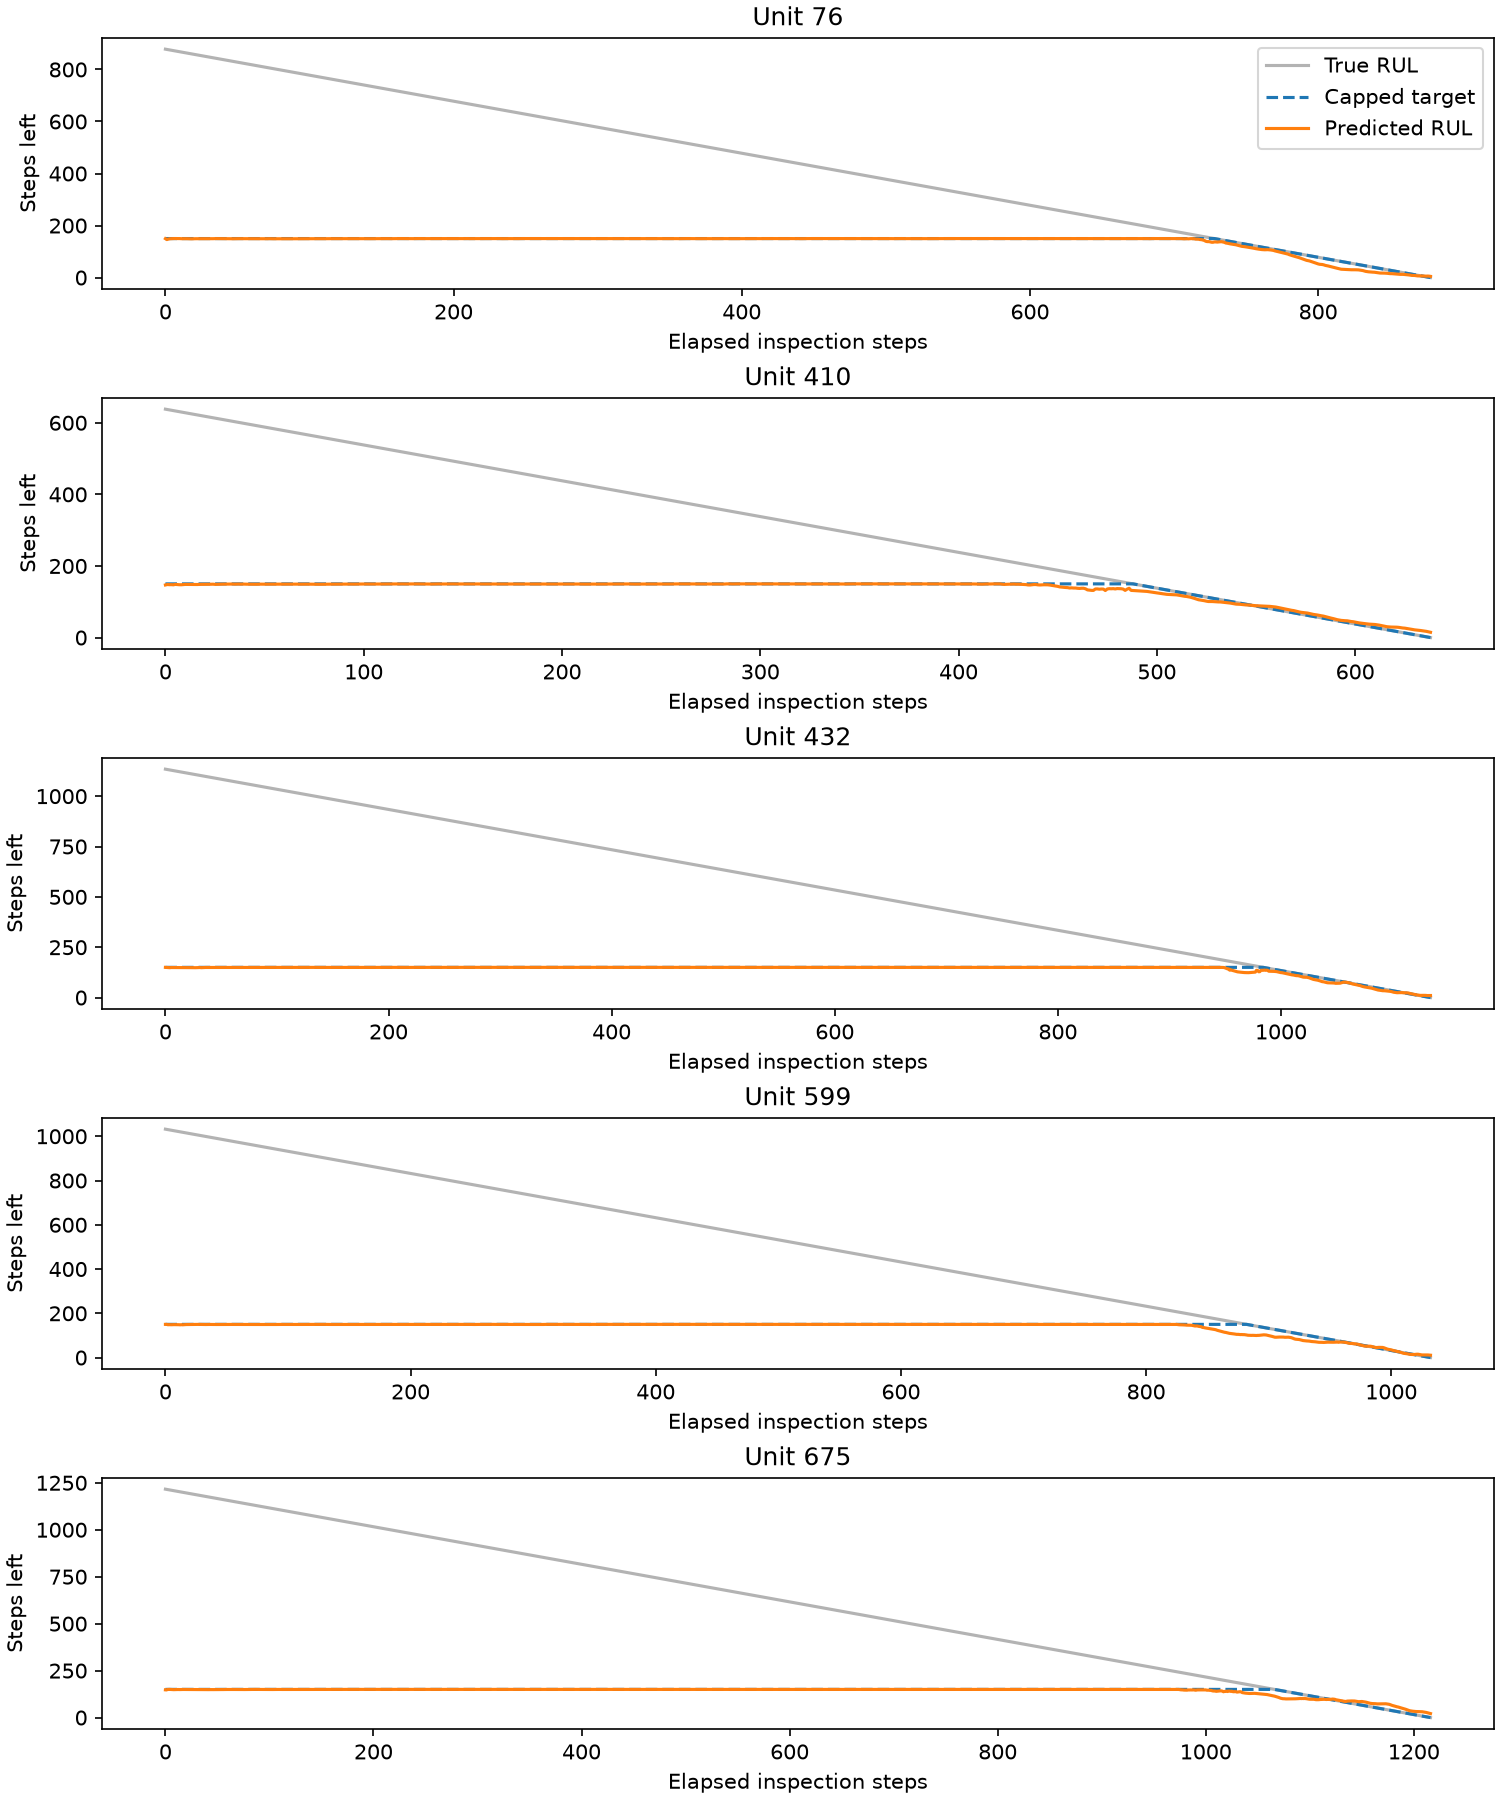
\includegraphics[width=\columnwidth,height=.50\textheight,keepaspectratio]{figures/figure-13.png}
\caption{RUL trajectories. Each panel shows the uncapped simulated remaining life, the target capped at 150 inspection steps, and the ensemble prediction for one of five test units.}
\label{fig:asset-13}
\end{figure}

\begin{figure}[!tp]
\centering
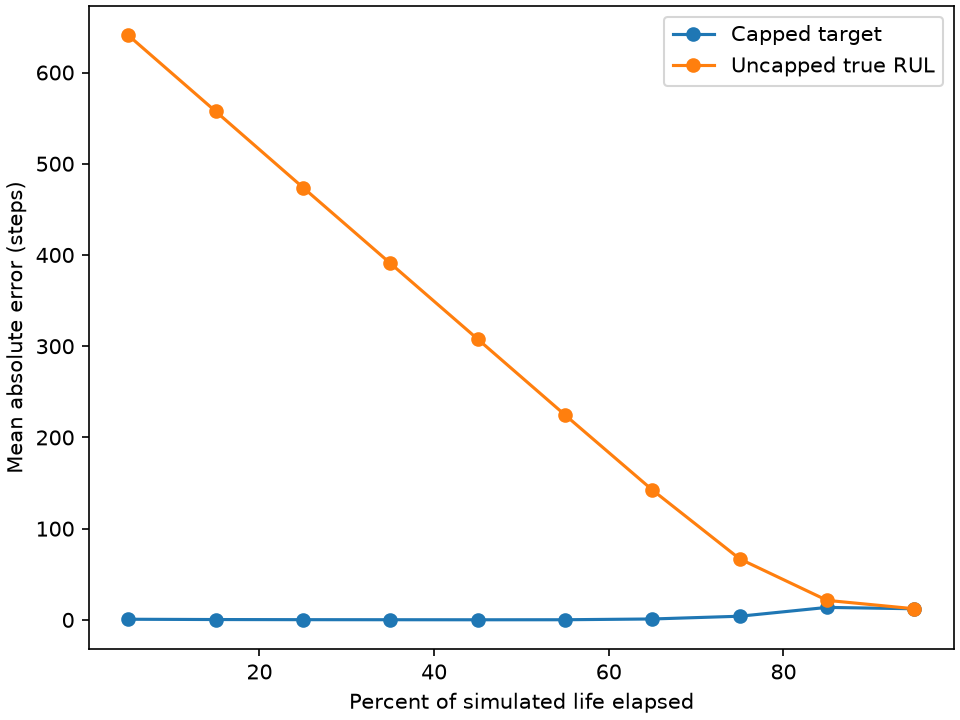
\includegraphics[width=\columnwidth,height=.43\textheight,keepaspectratio]{figures/figure-14.png}
\caption{RUL error by life stage. Test MAE by fraction of simulated lifetime elapsed, using capped and uncapped targets.}
\label{fig:asset-14}
\end{figure}

\begin{figure}[!tp]
\centering
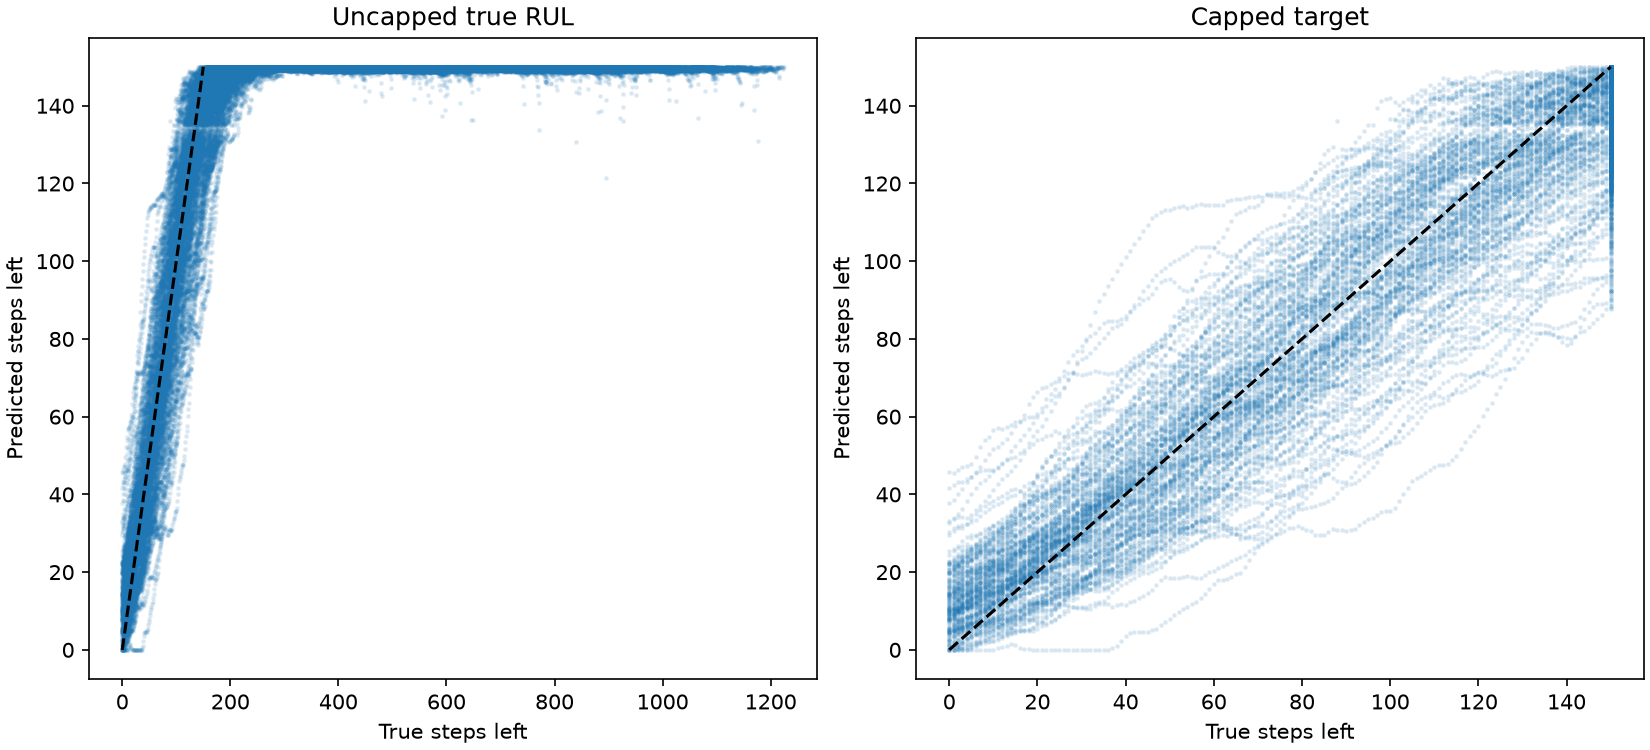
\includegraphics[width=\columnwidth,height=.43\textheight,keepaspectratio]{figures/figure-15.png}
\caption{Predicted versus true RUL. Scatter plots compare predictions to the uncapped and capped targets on simulated test histories.}
\label{fig:asset-15}
\end{figure}

\section{Discussion}

Few-shot adaptation improved the detector’s performance on double-layer PCB images. With 100 double-layer training images and 50 single-layer images, the detector reached 84.93\% mAP50 on the double-layer set, while its single-layer score fell to 72.81\%. Reusing all 100 original single-layer training images brought the scores to 83.01\% and 85.20\%, respectively. We chose the second checkpoint because it gave one detector a better balance across both board types. Because the runs used the same number of epochs, the larger training set also gave the model more updates per epoch.

The final detector’s performance varied by defect class. Short circuits reached 68.19\% AP50 on the double-layer set, where 61 of 147 labelled shorts were missed at the selected confidence threshold. Missing-hole detection performed well on the synthetic PKU layouts used to select the threshold and recovery settings. A visual review of double-layer DefectDet images found missing-hole alerts on existing holes and printed markings. The two datasets therefore show where the detector can help flag areas for inspection and where its predictions still need review.

On the simulated histories, predictions based on defect observations were more accurate than those based on elapsed time alone. The ensemble and the GRU had nearly identical average errors. The ensemble’s MAE rose from 3.28 steps across the capped test set to 10.58 steps in the final 50 steps before simulated failure, so the near-failure error is especially relevant when interpreting the estimate. The application demonstrates how a sequence of inspections can produce an updated RUL estimate. Its error figures apply to the simulated test histories.

\subsection{Comparison with Other Work}

Wang et al. [14] studied PCB defect detection with limited labelled examples. Their method combined features at multiple scales and achieved 69.52\% AP50 in the 10-shot setting and 78.86\% AP50 in the 30-shot setting. Our experiment used a different setup. We started with a detector trained on single-layer PCB images and adapted it using 50 or 100 labelled double-layer images in total. On the same 148-image double-layer comparison set, mAP50 rose from 0.00\% before adaptation to 79.41\% with 50 target images and 84.93\% with 100 target images. Both runs reused the same 50 single-layer training images. \href{https://doi.org/10.1109/ACCESS.2022.3228392}{Wang et al.}

On the nine-class DsPCBSD+ benchmark, Lv et al. [6] reported 84.80\% mAP50 for Co-DETR and 85.10\% mAP50 for YOLOv6-L6. Elsharkawy [15] reported 99.50\% mAP50 for YOLOv11-PCB on the Peking University PCB benchmark. Our final detector achieved 83.65\% mAP50 across five classes on single-layer PCB-Defect images and 84.46\% mAP50 across four classes on double-layer DefectDet images. The studies used different datasets, training budgets, and evaluated classes, so the published scores provide context for our results. The direct comparison in this study is the change on the same double-layer images before and after adaptation. \href{https://pmc.ncbi.nlm.nih.gov/articles/PMC11263390/\#Tab2}{Lv et al.} · \href{https://doi.org/10.1038/s41598-025-27415-w}{Elsharkawy}

\subsection{Observations}

Training on both board types helped retain single-layer performance. With 100 double-layer training images, increasing the number of original single-layer images from 50 to 100 raised single-layer mAP50 from 72.81\% to 85.20\%. With that change, double-layer mAP50 fell from 84.93\% to 83.01\%. The second model provided a better balance for inspecting both board types with one detector.

Short circuits remained difficult to detect on double-layer boards. The final detector missed 61 of 147 labelled shorts at the selected confidence threshold. During visual review, we also found missing-hole alerts on existing holes and printed markings. These cases show which predictions need the most attention during manual inspection.

RUL error was higher near simulated failure. The ensemble’s mean absolute error was 3.28 inspection steps against the 150-step capped target across the full test set and 10.58 steps when 50 or fewer steps remained. Fig.~\ref{fig:asset-13} shows how the predicted remaining life changed as five simulated units approached failure.

\section{Future Scope}

Additional multilayer PCB designs with verified layer counts would extend the detector evaluation. Grouping images by design would let us hold out entire designs for testing. Additional examples of short circuits, actual missing holes, intact holes, and printed markings would help test whether the detector can reduce missed defects and false alerts on unfamiliar boards.

Repeated inspections linked to recorded equipment failures would let us compare the model’s RUL estimates with the observed time to failure. These records could show whether changes in detected defects provide an early indication of equipment wear.

\section{Conclusion}

Our PCB inspection application uses one YOLO11s detector to locate six types of defects. We trained the base model on single-layer PCB images and adapted it using 100 labelled double-layer images alongside the original single-layer training images. The final detector achieved \textbf{83.65\% mAP50} across five evaluated classes on the single-layer set and \textbf{84.46\% mAP50} across four evaluated classes on the double-layer set. We evaluated missing-hole detection separately on the PKU dataset.

The application also uses saved inspection histories to estimate remaining useful life. On simulated test histories, the RUL model had a mean absolute error of \textbf{3.28 inspection steps} against the 150-step capped target and \textbf{10.58 steps} in the final 50 steps before simulated failure. The dashboard marks the detected defects in each image and updates the simulated remaining-life estimate as new inspections are recorded.

\FloatBarrier

\section*{References}

\begin{list}{}{\setlength{\leftmargin}{2em}\setlength{\labelwidth}{1.7em}\setlength{\itemsep}{.4ex}\footnotesize}

\item[[1]] A. J. Rashid, M. A. Ullah, A. Isfara, N. Ahmed, M. Mian, and M. M. Shalehin, “PCB-Defect: An Annotated Dataset for Surface Defect Detection in Printed Circuit Boards,” \textit{Mendeley Data}, version 1, 2025. \href{https://doi.org/10.17632/vdj74sngvn.1}{Single-layer dataset}

\item[[2]] A. Azam, M. M. Ishti, K. M. Shams, A. J. Rashid, and N. Ahmed, “DefectDet: An Annotated Dataset of Printed Circuit Boards with Surface Defects,” \textit{Mendeley Data}, version 1, 2026. \href{https://doi.org/10.17632/t9d9zs3bmb.1}{Double-layer dataset}

\item[[3]] W. Huang and P. Wei, “A PCB Dataset for Defects Detection and Classification,” \textit{arXiv}, 2019. \href{https://arxiv.org/abs/1901.08204}{PKU dataset paper}

\item[[4]] G. Jocher and J. Qiu, “Ultralytics YOLO11,” software, 2024. \href{https://docs.ultralytics.com/models/yolo11/}{Official documentation} · \href{https://github.com/ultralytics/ultralytics}{GitHub source code}

\item[[5]] Alpha-Ldz, “Lazarus — PCB Defect Detection \& Repair Station,” GitHub repository, weights-v1, pretrained checkpoint yolo11s-dspcbsd.pt. \href{https://github.com/Alpha-Ldz/lazarus}{GitHub repository}

\item[[6]] S. Lv \textit{et al}., “A dataset for deep learning based detection of printed circuit board surface defect,” \textit{Scientific Data}, vol. 11, art. no. 811, 2024. \href{https://doi.org/10.1038/s41597-024-03656-8}{DsPCBSD+ dataset article}

\item[[7]] I. Loshchilov and F. Hutter, “Decoupled Weight Decay Regularization,” in \textit{International Conference on Learning Representations (ICLR)}, 2019. \href{https://arxiv.org/abs/1711.05101}{AdamW paper}

\item[[8]] G. Ke \textit{et al}., “LightGBM: A Highly Efficient Gradient Boosting Decision Tree,” in \textit{Advances in Neural Information Processing Systems}, vol. 30, 2017. \href{https://proceedings.neurips.cc/paper/2017/hash/6449f44a102fde848669bdd9eb6b76fa-Abstract.html}{LightGBM paper}

\item[[9]] K. Cho \textit{et al}., “Learning Phrase Representations using RNN Encoder–Decoder for Statistical Machine Translation,” in \textit{Proceedings of EMNLP}, pp. 1724–1734, 2014. \href{https://aclanthology.org/D14-1179/}{Original GRU paper}

\item[[10]] T. Akiba, S. Sano, T. Yanase, T. Ohta, and M. Koyama, “Optuna: A Next-generation Hyperparameter Optimization Framework,” in \textit{Proceedings of the 25th ACM SIGKDD International Conference on Knowledge Discovery \& Data Mining}, pp. 2623–2631, 2019. \href{https://doi.org/10.1145/3292500.3330701}{Optuna paper}

\item[[11]] A. Paszke \textit{et al}., “PyTorch: An Imperative Style, High-Performance Deep Learning Library,” in \textit{Advances in Neural Information Processing Systems}, vol. 32, 2019. \href{https://papers.nips.cc/paper_files/paper/2019/hash/bdbca288fee7f92f2bfa9f7012727740-Abstract.html}{PyTorch paper}

\item[[12]] F. Pedregosa \textit{et al}., “Scikit-learn: Machine Learning in Python,” \textit{Journal of Machine Learning Research}, vol. 12, pp. 2825–2830, 2011. \href{https://www.jmlr.org/papers/v12/pedregosa11a.html}{Scikit-learn paper}

\item[[13]] A. Saxena, K. Goebel, D. Simon, and N. Eklund, “Damage propagation modeling for aircraft engine run-to-failure simulation,” in \textit{International Conference on Prognostics and Health Management}, pp. 1–9, 2008. \href{https://doi.org/10.1109/PHM.2008.4711414}{Source of the asymmetric RUL scoring method}

\item[[14]] H. Wang, J. Xie, X. Xu, and Z. Zheng, “Few-Shot PCB Surface Defect Detection Based on Feature Enhancement and Multi-Scale Fusion,” \textit{IEEE Access}, vol. 10, pp. 129911–129924, 2022.\href{https://doi.org/10.1109/ACCESS.2022.3228392}{ DOI}

\item[[15]] Z. F. Elsharkawy, “Enhanced YOLOv11 framework for high precision defect detection in printed circuit boards,” \textit{Scientific Reports}, vol. 15, art. no. 42550, 2025.\href{https://doi.org/10.1038/s41598-025-27415-w}{ DOI}

\end{list}

\FloatBarrier

\end{document}
